\noindent Als Voraussetzung für die digitale Signalverarbeitung müssen die analogen, zeit- und wertkonti-nuierlichen Signale so gewandelt werden, dass sie abgespeichert und weiter verarbeitet werden können. Diese Wandlung wird Digitalisierung genannt.\medskip

\noindent Dazu muss das Signal einerseits zeitlich quantisiert werden, da nur endlich viele Werte verarbei-tet werden können. Zu diskreten Zeitpunkten wird dabei der aktuelle Wert des Signals erfasst oder abgetastet. Die Abstände zwischen den Zeitpunkten, zu denen die Werte erfasst werden, sind üblicherweise äquidistant, also immer gleich groß. Die erfassten Werte werden Abtastwerte genannt. Außerdem muss die Amplitude des Signals bestimmt werden, was nur in einem be-grenzten Bereich und mit einer definierten Auflösung oder Quantisierung möglich ist. \medskip

\noindent Nach einer kurzen Darstellung zum Umgang mit Quantisierungsfehlern bei der Amplitude wird in diesem Kapitel die Zeitdiskretisierung betrachtet, da eine falsche Zeitdiskretisierung fatale Auswirkungen auf die folgende Signalverarbeitung hat. Zunächst wird allgemein erklärt, wie die ideale Abtastung von Signalen mathematisch beschrieben werden kann. Hierbei wird deutlich, warum das Spektrum eines abgetasteten Signals immer periodisch ist. Anhand der Periodizität des Spektrums wird das Abtasttheorem von Shannon eingeführt. Es besagt, dass die Abtastfre-quenz bei bandbegrenzten Signalen mehr als doppelt so groß sein muss, wie die größten Fre-quenzanteile im Signal. Mit dem Anti-Aliasing-Tiefpass wird eine Methode vorgestellt, wie Sig-nale ohne Bandbegrenzung gefiltert werden können, um das Abtasttheorem zu erfüllen. \medskip

\noindent Da die ideale Abtastung von Signalen nur in der Theorie existiert und in der Praxis so nicht di-rekt angewandt werden kann, wird darüber hinaus die reale Abtastung mathematisch beschrie-ben und die dadurch entstehenden Signalverzerrungen erläutert. Auch hier gibt es die Möglich-keit, die Effekte durch die geschickte Anwendung von Filtern zu kompensieren.


\subsection{Quantisierungsfehler der Amplitude}

\noindent Bei der Digitalisierung von Signalen muss die Amplitude einer festen Quantisierungsstufe zugeordnet werden. Entscheidend für die Quantisierung des Signals ist die Auflösung des Analog-Digital-Wandlers (AD-Wandlers), die üblicherweise in Bit angegeben wird. Beispielsweise wird mit einem 12-Bit-AD-Wandler ein definierter Messbereich in 2${}^{12}$ = 4096 Intervalle eingeteilt. Bei einem Messbereich von 5 V ergäben sich demnach bei einer Auflösung von 12 Bit Quantisierungsstufen von. 

\begin{equation}\label{eq:twoone}
\Delta U=\frac{5{ \; V}}{2^{12} } =\frac{5{ \; V}}{4096} =1.2\; mV
\end{equation}


\noindent In der Praxis wird die Quantisierung der Amplitude gerne vernachlässigt, weil die entstehenden Fehler durch eine hohe Auflösung des verwendeten Analog-Digital-Wandlers klein gehalten werden können. Die existierende Abweichung zwischen dem wertdiskreten und wertkontinuierlichen Signal wird als Quantisierungsfehler modelliert. Bild \ref{fig:Quantisierungsfehler} verdeutlicht den Quantisierungsfehler an zwei Beispielen.

\clearpage

\begin{figure}[H]
  \centerline{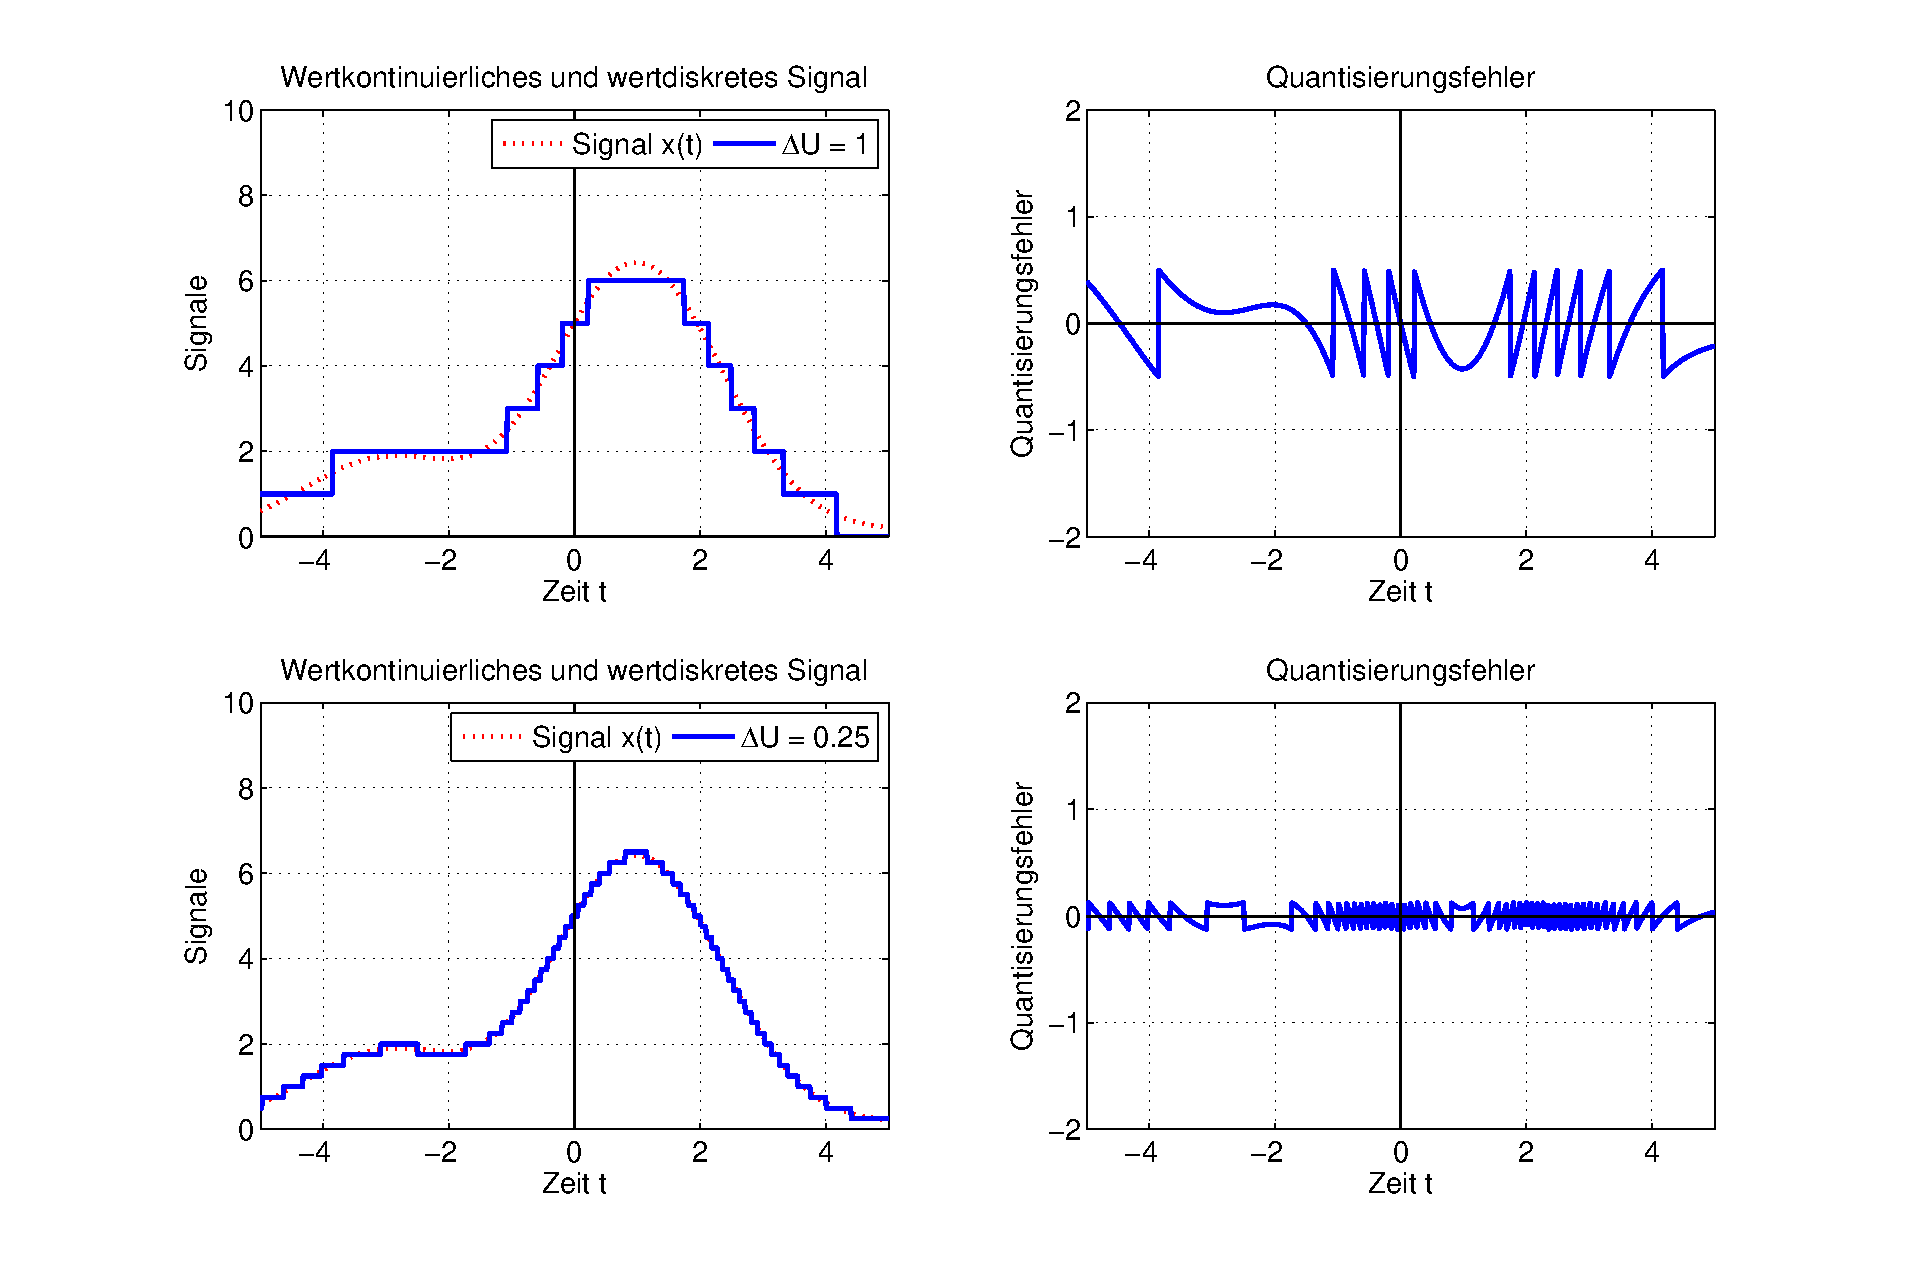
\includegraphics[width=1\textwidth]{Kapitel1/Bilder/image1}}
  \caption{Darstellung des Quantisierungsfehlers (Quantisierungsrauschens)}
  \label{fig:Quantisierungsfehler}
\end{figure}

\noindent Der Quantisierungsfehler ergibt sich aus der Differenz zwischen dem wertkontinuierlichen und dem wertdiskreten Signal. Je feiner die Auflösung des AD-Wandlers ist, desto geringer ist der Abstand zwischen dem kontinuierlichen und dem quantisierten Signal. Da die Abweichung einen zufälligen Verlauf zu haben scheint, wird dieser Fehler als Quantisierungsrauschen bezeichnet und als zufälliger Fehler oder zufälliges Störsignal behandelt. Der Umgang mit zufälligen Signalen ist Gegenstand des Teils C dieser Buchreihe, der Quantisierungsfehler wird an dieser Stelle deshalb nicht weiter vertieft.

\clearpage


\subsection{Vorüberlegungen zur zeitlichen Diskretisierung}

\noindent Die grundlegende Frage bei der zeitlichen Abtastung von Signalen ist, in welchen Zeitabständen T$_{A}$ beziehungsweise mit welcher Abtastfrequenz f$_{A}$ ein Signal erfasst werden muss. Die Bedeutung dieser Frage wird an einem Beispiel erläutert. \bigskip

\noindent
\colorbox{lightgray}{%
\arrayrulecolor{white}%
\renewcommand\arraystretch{0.6}%
\begin{tabular}{ wl{16.5cm} }
{\fontfamily{phv}\selectfont{Beispiel: Abtastwerte} }
\end{tabular}%
}\bigskip

\noindent Bild \ref{fig:AbtastwerteUnterschiedlicheAbtastzeiten} zeigt Abtastwerte eines Signals, das mit unterschiedlichen Abtastzeiten T$_{A}$ abgetastet wird. Die Abtastwerte sind jeweils über Geradenabschnitte miteinander verbunden. Das Signal scheint davon abzuhängen, wie es abgetastet wird.

\begin{figure}[H]
  \centerline{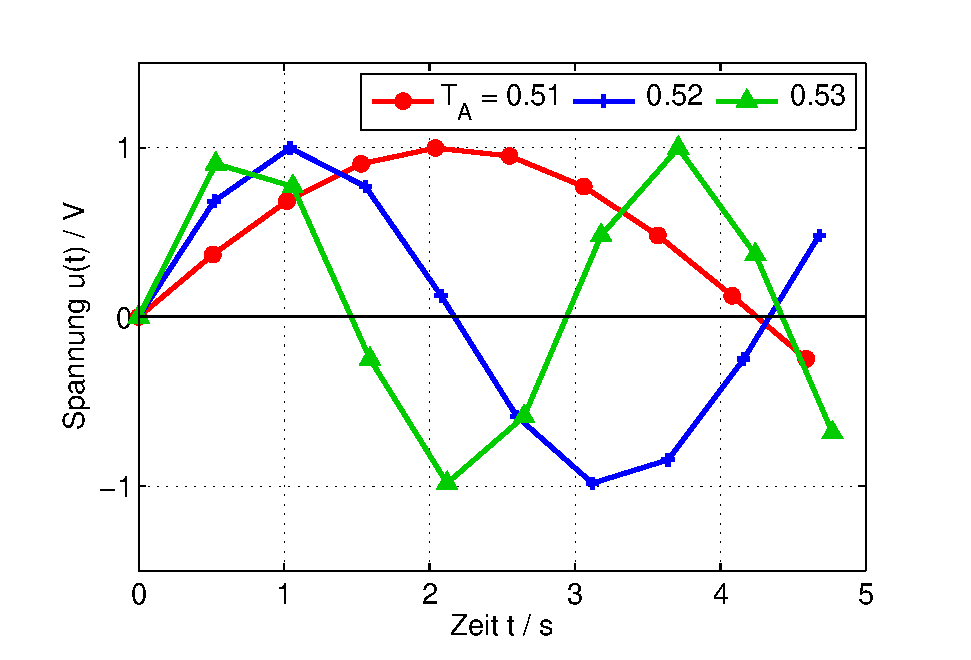
\includegraphics[width=0.5\textwidth]{Kapitel1/Bilder/image2}}
  \caption{Darstellung der Abtastwerte eines Signals, das mit unterschiedlichen Abtastzeiten T$_{A}$ abgetastet wird}
  \label{fig:AbtastwerteUnterschiedlicheAbtastzeiten}
\end{figure}


\noindent Das zugrunde liegende Signal ist sinusförmig und wird mit der Funktion

\begin{equation}\label{eq:twotwo}
u\left(t\right)=1{\rm \; }V\cdot \sin \left(2\cdot \pi \cdot 6\cdot t\right)
\end{equation}

\noindent beschrieben. D Der Vergleich der Abtastwerte mit dem Signal u(t) in Bild 2.3zeigt, dass alle in Bild 2.2 dargestellten abgetasteten Signale falsch oder zumindest irreführend sind.

\begin{figure}[H]
  \centerline{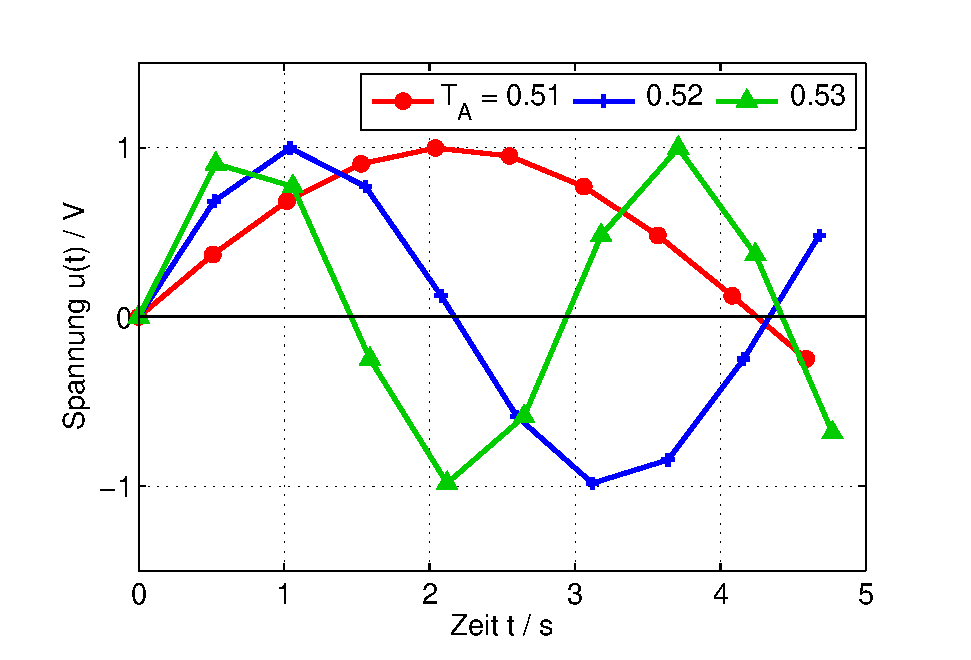
\includegraphics[width=0.5\textwidth]{Kapitel1/Bilder/image2}}
  \caption{Vergleich der Abtastwerte eines harmonischen Signals mit dem Originalsignal}
  \label{fig:Vergleich}
\end{figure}

\noindent Die Abtastwerte liegen auf einer Schwingung mit wesentlich höherer Frequenz und geben nicht das eigentliche Signal wieder. Daraus kann die Schlussfolgerung gezogen werden, dass beim Abtasten Regeln eingehalten werden müssen, um das Signal richtig rekonstruieren zu können. Diese Überlegung wird zu dem Abtasttheorem führen. 

\clearpage

\noindent Vor der allgemeinen Herleitung des Abtasttheorems werden die Abtastwerte eines harmonischen Signals x(t) mit einer Frequenz f$_{0}$ analysiert. Das Signal ist definiert als 

\begin{equation}\label{eq:twothree}
x\left(t\right)=\sin \left(2\cdot \pi \cdot f_{0} \cdot t\right)
\end{equation}

\noindent Das Signal wird mit einer Abtastzeit T${}_{A}$ abgetastet, sodass sich an den ganzzahligen Vielfachen k der Abtastzeit t~=~k$\cdot$T${}_{A}$ die Werte ergeben zu

\begin{equation}\label{eq:twofour}
x\left[k\right]=x\left(k\cdot T_{A} \right)=\sin \left(2\cdot \pi \cdot f_{0} \cdot k\cdot T_{A} \right)
\end{equation}

\noindent Die Abtastwerte der Signalfolge stimmen mit einer Signalfolge überein, die sich aus der Abtastung eines harmonischen Signals mit einer Frequenz f${}_{0}$ und dem Vielfachen der Abtastfrequenz n$\cdot$f${}_{A}$ ergibt. Einsetzen der Bedingungen ergibt 

\begin{equation}\label{eq:twofive}
\begin{split}
\sin \left(2\cdot \pi \cdot \left(f_{0} +n\cdot f_{A} \right)\cdot k\cdot T_{A} \right) 
& = \sin \left(2\cdot \pi \cdot \left(f_{0} \cdot k\cdot T_{A} +\frac{n}{T_{A} } \cdot k\cdot T_{A} \right)\right) \\ 
& = \sin \left(2\cdot \pi \cdot f_{0} \cdot k\cdot T_{A} +2\cdot \pi \cdot n\cdot k\right)=\sin \left(2\cdot \pi \cdot f_{0} \cdot k\cdot T_{A} \right)  
\end{split}
\end{equation}

\noindent Der Faktor n$\cdot$k ist dabei ein ganzzahliger Wert. Das bedeutet, dass die Abtastwerte, die ein Signal der Frequenz f${}_{0}$ repräsentieren, genau dieselben sind wie diejenigen, die sich beim Abtasten eines Signals der Frequenz f${}_{0}$ und einem Vielfachen der Abtastfrequenz f${}_{A}$ ergeben. Nach der Abtastung kann also nicht zwischen Signalen der Frequenz f${}_{0}$ und f$_{0}$ + n $\cdot$f$_{A}$ unterschieden werden. Bild \ref{fig:AbtastwerteHarmonischesSignal} stellt die Signal- und Abtastwerte für ein Beispiel dar.

\begin{figure}[H]
  \centerline{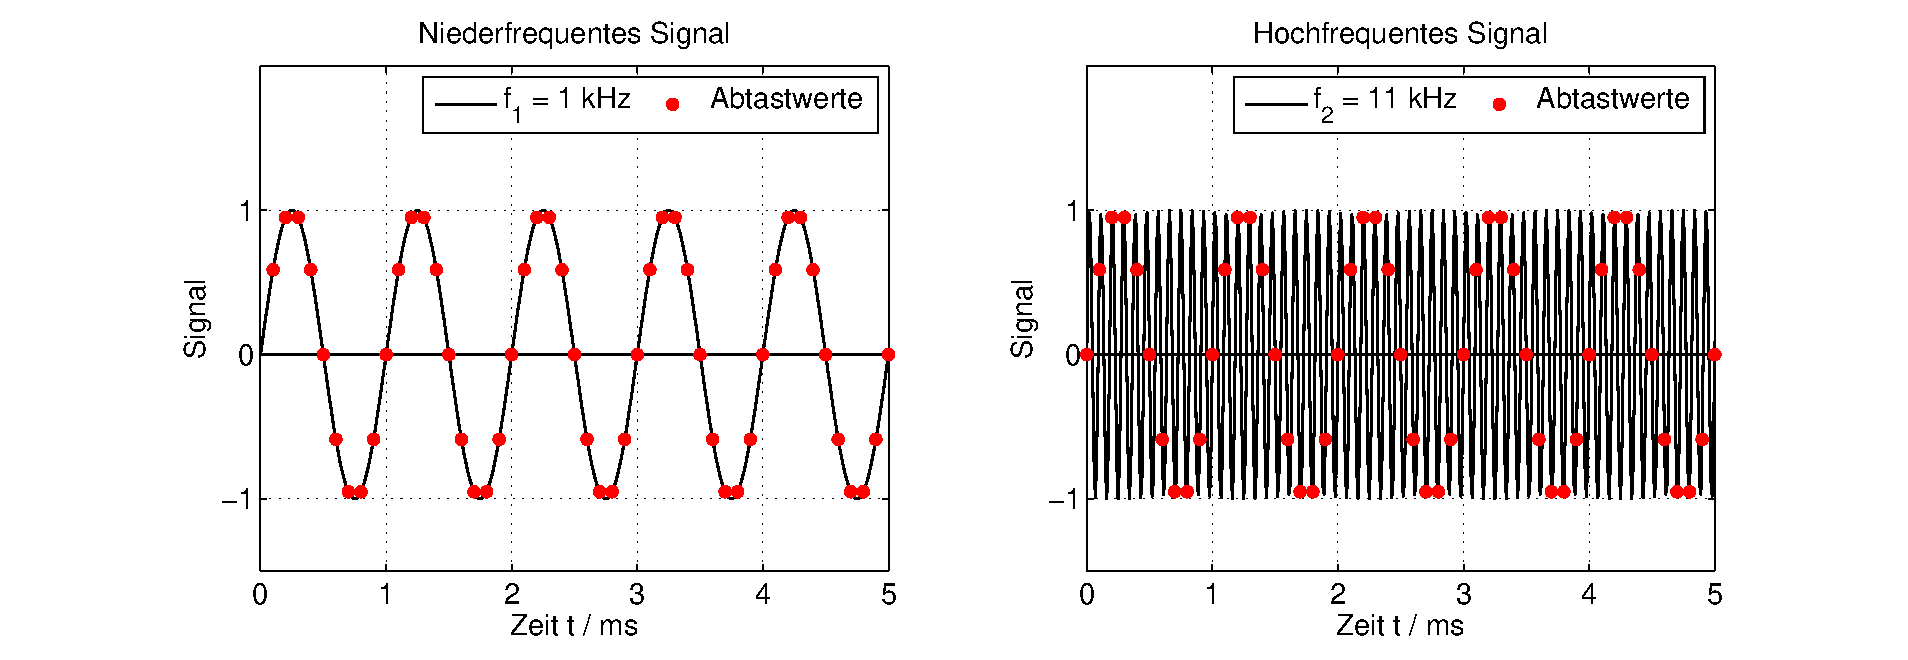
\includegraphics[width=1\textwidth]{Kapitel1/Bilder/image4}}
  \caption{Abtastwerte für ein harmonisches Signal mit der Frequenz f${}_{01}$ = 1 kHz und f${}_{02}$ = 11 kHz}
  \label{fig:AbtastwerteHarmonischesSignal}
\end{figure}

\noindent Das Signal wird mit einer Frequenz f${}_{A}$ = 10 kHz abgetastet. Die Abtastwerte sind für ein Signal mit einer Frequenz f${}_{1}$~=~1~kHz und einem Signal mit einer Frequenz f${}_{2}$ = 11 kHz identisch.\newline

\noindent Der hier für harmonische Schwingungen dargestellte Sachverhalt gilt auch für nicht harmonische Signale, da sie sich mit der Fourier-Transformation auf harmonische Signale zurückführen lassen. Dieser Effekt macht es erforderlich, den Abtastvorgang mathematisch zu beschreiben und Bedingungen für den Abtastvorgang zu definieren, unter denen ein abgetastetes Signal rekonstruiert werden kann.

\clearpage


\subsection{Ideale Abtastung und ideale Rekonstruktion}

\noindent Für die systemtheoretische Behandlung der digitalen Signalverarbeitung ist es erforderlich, die Abtastung und die Rekonstruktion des Signals mathematisch ideal zu beschreiben. Aus dieser Beschreibung wird anschlie{\ss}end das Abtasttheorem hergeleitet.


\subsubsection{Mathematische Beschreibung der idealen Abtastung}

\noindent Um die Abtastung eines Signals mathematisch beschreiben zu können, wird eine sogenannte Abtastfunktion a(t) definiert. Da bei der idealen Abtastung Werte des analogen Signals zu diskreten Zeitpunkten erfasst werden, bietet sich eine Folge von Impulsen als Abtastfunktion an. Diese Abtastfunktion a(t) ist mathematisch definiert als 

\begin{equation}\label{eq:twosix}
a\left(t\right)=\sum _{k=-\infty }^{\infty }\delta \left(t-k\cdot T_{A} \right) 
\end{equation}

\noindent Die Abtastfunktion wird mit dem analogen Signal x(t) multipliziert. Da die Impulsfolge nur zu den Zeitpunkten k$\cdot$T$_{A}$ ungleich null ist, genügt es, die Funktion x(t) nur zu diesen Zeitpunkten zu betrachten. Es ergibt sich als Darstellung für das ideal abgetastete Signal x$_{A}$(t)

\begin{equation}\label{eq:twoseven}
x_{A} \left(t\right)=x\left(t\right)\cdot a\left(t\right)=x\left(t\right)\cdot \sum _{k=-\infty }^{\infty }\delta \left(t-k\cdot T_{A} \right) =\sum _{k=-\infty }^{\infty }x\left(k\cdot T_{A} \right)\cdot \delta \left(t-k\cdot T_{A} \right)
\end{equation}

\noindent Bild \ref{fig:AbtastprozessIdealSignal} verdeutlicht die mathematische Beschreibung der Signale grafisch. Dabei werden die unendlich gro{\ss}en Impulse als Pfeile dargestellt, ihre Höhe repräsentiert das Gewicht des jeweiligen Impulses.

\begin{figure}[H]
  \centerline{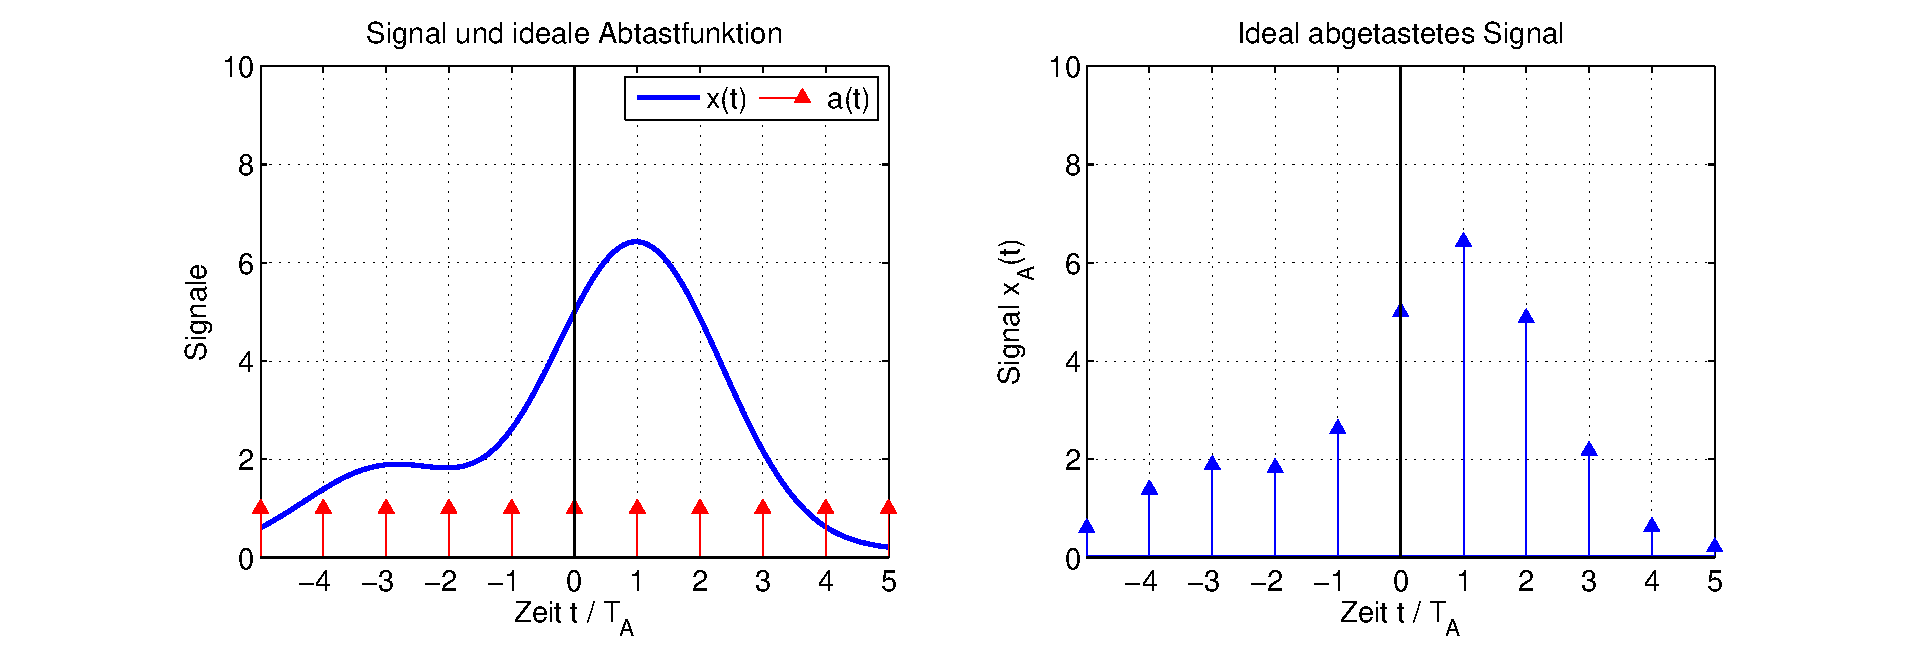
\includegraphics[width=1\textwidth]{Kapitel1/Bilder/image5}}
  \caption{Darstellung der Signale im idealen Abtastprozess
}
  \label{fig:AbtastprozessIdealSignal}
\end{figure}

\noindent Wird dieser Vorgang im Frequenzbereich betrachtet, wird deutlich, dass durch das Abtasten das Spektrum des Signals periodisch wird. Im Zeitbereich wird das Signal x(t) mit der Abtastfunktion a(t) multipliziert. Der Multiplikation im Zeitbereich entspricht eine Faltung im Frequenzbereich. Damit muss im Frequenzbereich das Spektrum des Signals X($\omegaup$) mit dem Spektrum der Abtastfunktion A($\omegaup$) gefaltet werden. Hierfür wird zunächst das Spektrum der Abtastfunktion errechnet.

\begin{equation}\label{eq:twoeight}
\Im \left\{a\left(t\right)\right\}=\Im \left\{\sum _{k=-\infty }^{\infty }\delta \left(t-k\cdot T_{A} \right) \right\}
\end{equation}

\noindent Die Gleichung kann als Fourier-Reihe dargestellt werden und in den folgenden Ausdruck umgeformt werden

\begin{equation}\label{eq:twonine}
\Im \left\{a\left(t\right)\right\}=\Im \left\{\sum _{k=-\infty }^{\infty }\delta \left(t-k\cdot T_{A} \right) \right\}=\frac{2\cdot \pi }{T_{A} } \cdot \sum _{k=-\infty }^{\infty }\delta \left(\omega -k\cdot \frac{2\cdot \pi }{T_{A} } \right) =\frac{2\cdot \pi }{T_{A} } \cdot \sum _{k=-\infty }^{\infty }\delta \left(\omega -k\cdot \omega _{A} \right) 
\end{equation}

\noindent Dies bedeutet, dass die Abtastfunktion auch im Frequenzbereich einer Impulsfolge entspricht, wobei der Abstand der Impulse proportional zur Abtastfrequenz

\begin{equation}\label{eq:twoten}
\omega _{A} =2\cdot \pi \cdot f_{A} =\frac{2\cdot \pi }{T_{A} }
\end{equation}

\noindent ist. Über die Faltungsbeziehung ergibt sich für die abgetastete Funktion x$_{A}$(t) im Frequenzbereich 

\begin{equation}\label{eq:twoeleven}
\begin{split}
X_{A} \left(\omega \right) & = \frac{1}{2\cdot \pi } \cdot \left(X\left(\omega \right)*\left(\frac{2\cdot \pi }{T_{A} } \cdot \sum _{k=-\infty }^{\infty }\delta \left(\omega -k\cdot \frac{2\cdot \pi }{T_{A} } \right) \right)\right) \\ 
& = \frac{1}{T_{A} } \cdot \sum _{k=-\infty }^{\infty }X\left(\omega -k\cdot \frac{2\cdot \pi }{T_{A} } \right) =\frac{1}{T_{A} } \cdot \sum _{k=-\infty }^{\infty }X\left(\omega -k\cdot \omega _{A} \right)    
\end{split}
\end{equation}

\noindent Die Eine Abtastung mit einer idealen Impulsreihe der idealen Abtastfunktion führt demnach zu einer in $\omega{A}$ periodischen Fortsetzung des Spektrums X($\omega$) des kontinuierlichen Zeitsignals x(t) und zu einer Multiplikation mit dem Faktor 1/T${}_{A}$. Bild \ref{fig:AbtastprozessIdealSpektrum} stellt die Spektren im idealen Abtastprozess schematisch dar.

\begin{figure}[H]
  \centerline{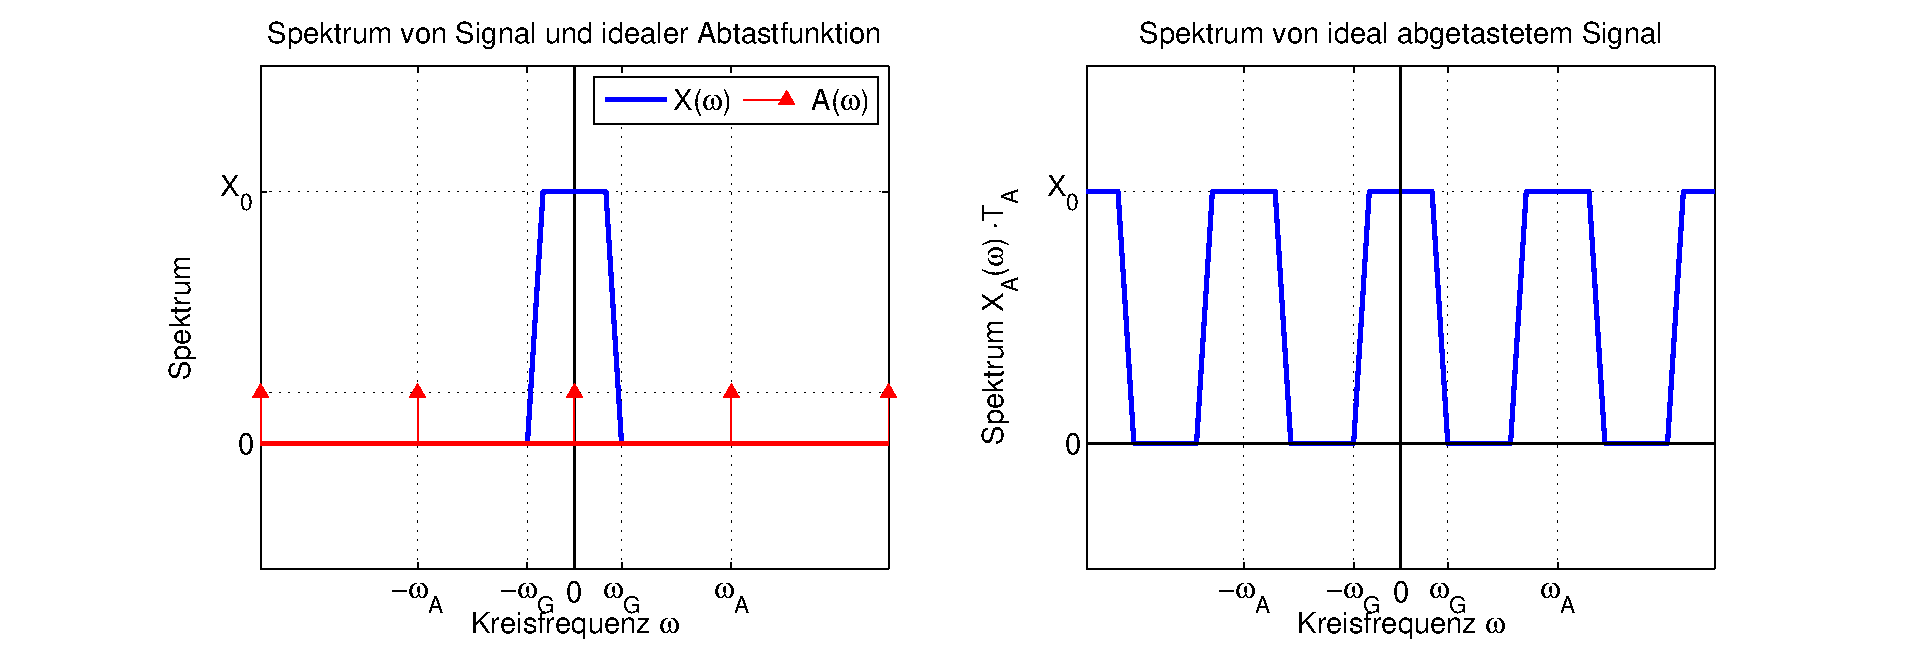
\includegraphics[width=1\textwidth]{Kapitel1/Bilder/image6}}
  \caption{Darstellung der Spektren im idealen Abtastprozess}
  \label{fig:AbtastprozessIdealSpektrum}
\end{figure}

\noindent Die periodische Wiederholung des Spektrums ist dafür verantwortlich, dass die Abtastwerte von zu langsam abgetasteten Signalen mit den Frequenzen f${}_{0}$ und f${}_{0}$ + n$.$f${}_{A}$ nicht unterschieden werden können. Die mathematische Herleitung bestätigt damit den in Bild \ref{fig:AbtastprozessIdealSpektrum} dargestellten Sachverhalt.

\noindent Der ursprüngliche Frequenzbereich des Signals x(t) mit dem Frequenzbereich - $\omega_{G}$ $\leq$ $\omega$ $\leq$ $\omega_{G}$ wird als Basisband des Signals bezeichnet. Durch den Abtastvorgang wird das Basisband periodisch in $\omega_{A}$ wiederholt.


\subsubsection{Ideale Rekonstruktion eines Signals}

\noindent Da bei der idealen Abtastung das Spektrum eines Signals periodisch wiederholt und mit dem Faktor 1/T${}_{A}$ multipliziert wird, liegt es auf der Hand, die Wiederholung des Spektrums durch eine entsprechende Filterung zu eliminieren. Durch eine hier ideal angenommene Tiefpass-Funktion mit einer Bandbreite Grenzfrequenz von $\omega_{A}$/2 kann das sogenannte Basisband, also das ursprüngliche Spektrum der Zeitfunktion, isoliert werden. Bild \ref{fig:RekonstruktionIdeal} verdeutlicht den Filterprozess.

\begin{figure}[H]
  \centerline{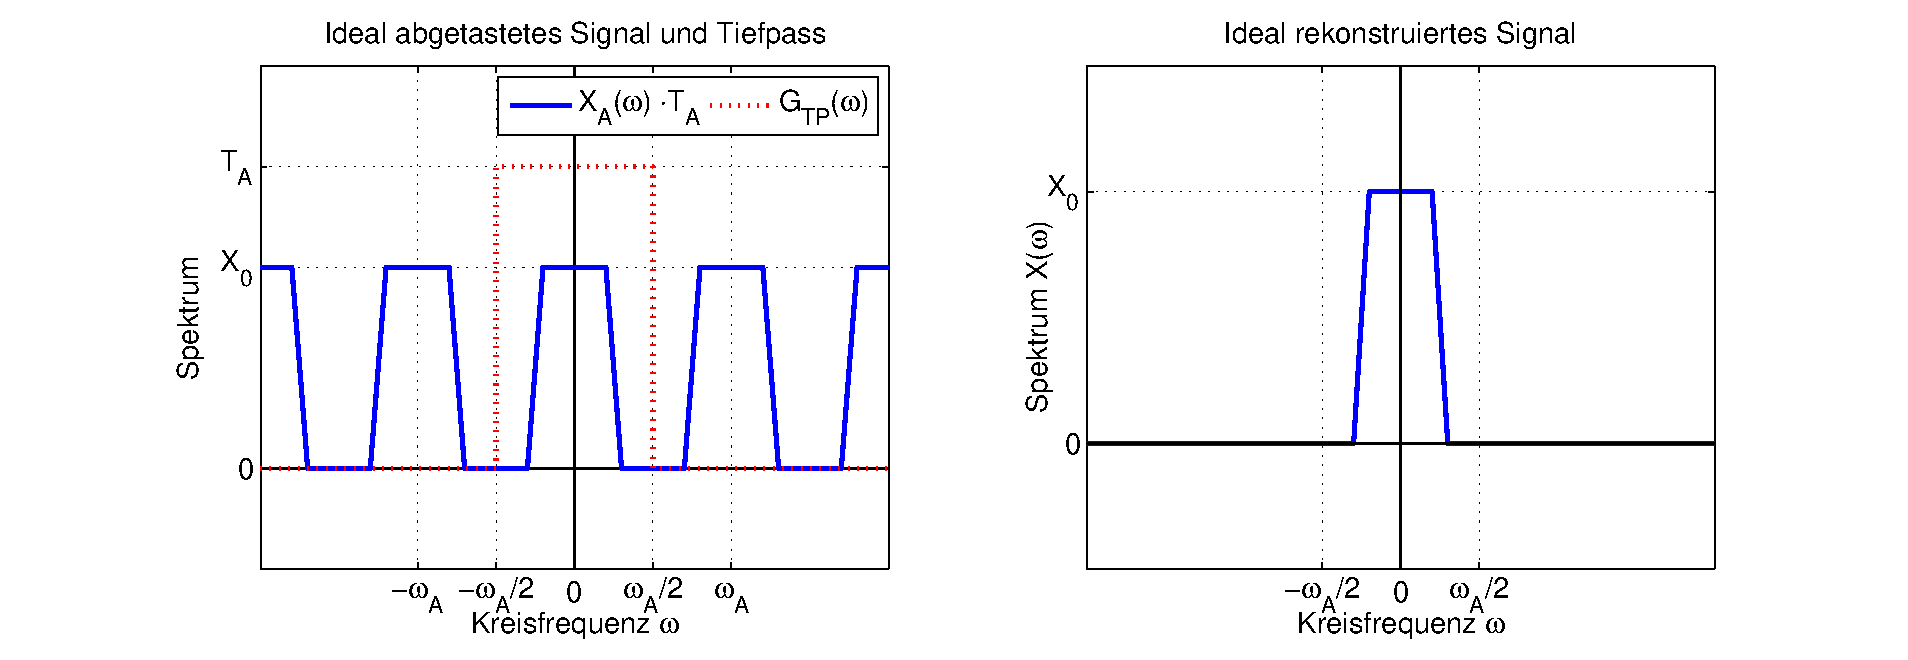
\includegraphics[width=1\textwidth]{Kapitel1/Bilder/image7}}
  \caption{Rekonstruktion des Spektrums der Zeitfunktion durch ideale Tiefpass-Filterung, idealisierte Tiefpass-Funktion gestrichelt dargestellt}
  \label{fig:RekonstruktionIdeal}
\end{figure}

\noindent Mathematisch gesehen muss das Spektrum mit einer idealen Tiefpass-Filterfunktion und dem Faktor T${}_{A}$ multipliziert werden. Das Spektrum ergibt sich damit zu

\begin{equation}\label{eq:twotwelve}
\begin{split}
X\left(\omega \right) & = G_{TP} \left(\omega \right)\cdot X_{A} \left(\omega \right)=T_{A} \cdot \left(\sigma \left(\omega +\frac{\omega _{A} }{2} \right)-\sigma \left(\omega -\frac{\omega _{A} }{2} \right)\right)\cdot \frac{1}{T_{A} } \cdot \sum _{k=-\infty }^{\infty }X\left(\omega -k\cdot \omega _{A} \right)\\
& =
\end{split}
\end{equation}


\noindent Die ideale Rekonstruktion kann auch im Zeitbereich durchgeführt werden. Der Multiplikation im Frequenzbereich entspricht im Zeitbereich die Faltung der entsprechenden Zeitfunktionen. Die Impulsantwort g$_{TP}$(t) der Filterfunktion G$_{TP}$($\omega$) ist nach den Rechenregeln der Fourier-Transformation 

\begin{equation}\label{eq:twothirteen}
g_{TP} \left(t\right)=\frac{T_{A} }{\pi } \cdot \frac{\sin \left(\frac{\omega _{A} }{2} \cdot t\right)}{t}
\end{equation}

\noindent Die Funktion Impulsantwort de Tiefsses ist in Bild \ref{fig:RekonstruktionIdealSignal} dargestellt. Zum Zeitpunkt t = 0 ist die Funktion 1, zu den Zeitpunkten k$\cdot$T${}_{A}$ ist die Funktion null.

\begin{figure}[H]
  \centerline{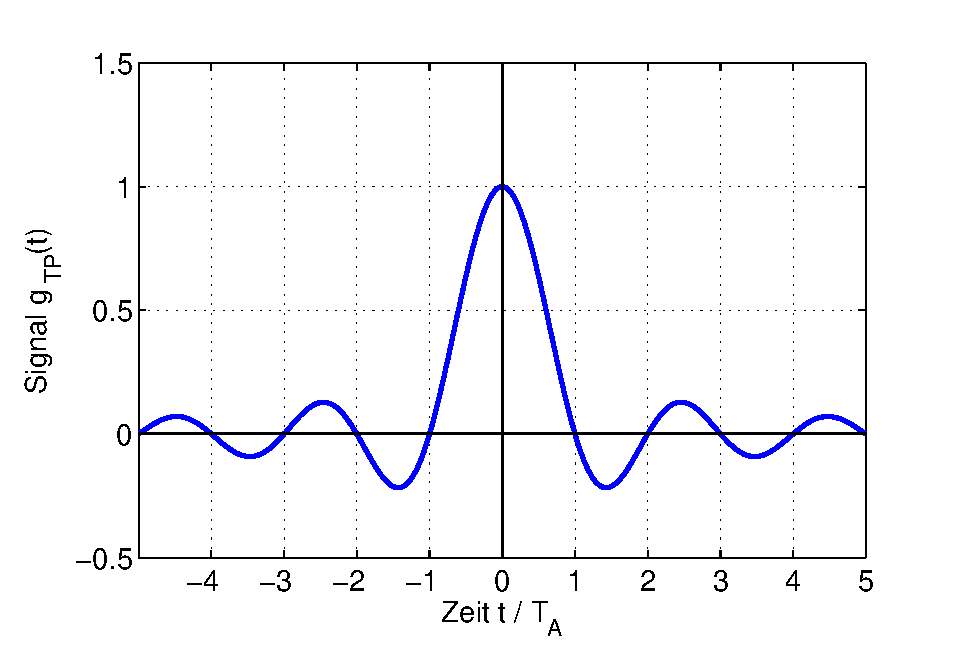
\includegraphics[width=0.5\textwidth]{Kapitel1/Bilder/image8}}
  \caption{Impulsantwort des idealen Tiefpass-Filters zur Rekonstruktion}
  \label{fig:RekonstruktionIdealSignal}
\end{figure}

\noindent Das Signal x(t) berechnet sich über das Faltungsintegral. Da die Faltung einer Funktion x(t) mit einem Impuls an der Stelle t$_{0}$ die Funktion an die Stelle x(t - t$_{0}$) verschiebt, ergibt sich

\begin{equation}\label{eq:twofourteen}
\begin{split}
x\left(t\right) & = g_{TP} \left(t\right)*x_{A} \left(t\right)=\frac{T_{A} }{\pi } \cdot \frac{\sin \left(\frac{\omega _{A} }{2} \cdot t\right)}{t} *\sum _{k=-\infty }^{\infty }x\left(k\cdot T_{A} \right)\cdot \delta \left(t-T_{A} \cdot k\right) \\ {} 
\end{split}
\end{equation}

\noindent Das Signal setzt sich aus der Summe von Termen g$_{TP}$(t) zusammen, die jeweils um k$\cdot$T${}_{A}$ verschoben sind und mit dem Gewicht x(k$\cdot$T${}_{A}$) multipliziert werden. Bild \ref{fig:RekonstruktionIdealSignalimZeit} stellt die Rekonstruktion im Zeitbereich dar.

\begin{figure}[H]
  \centerline{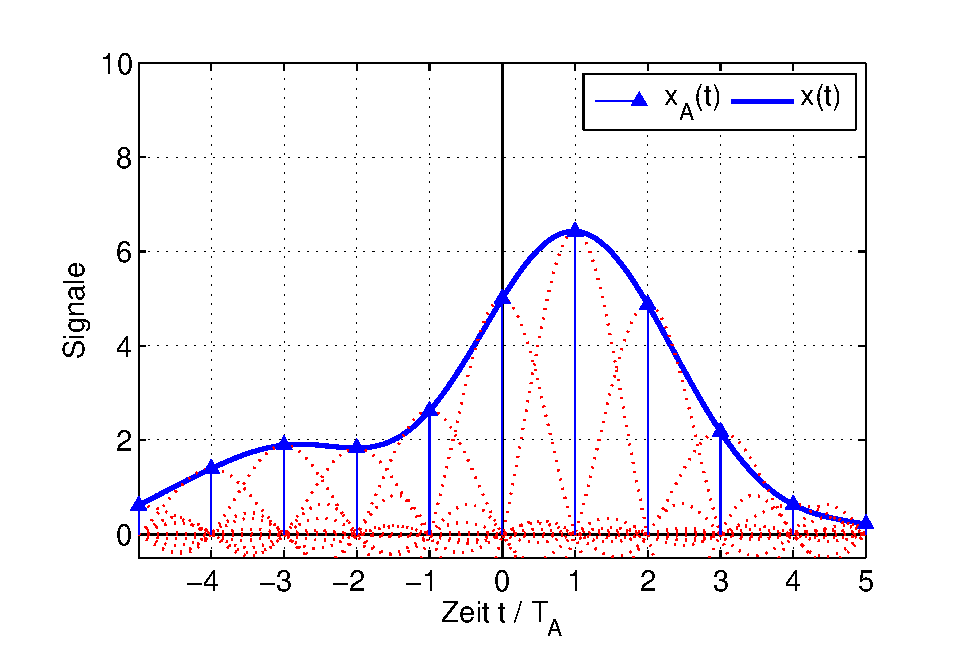
\includegraphics[width=0.5\textwidth]{Kapitel1/Bilder/image9}}
  \caption{Rekonstruktion eines ideal abgetasteten Signals im Zeitbereich}
  \label{fig:RekonstruktionIdealSignalimZeit}
\end{figure}


\noindent Das Ergebnis der Überlagerung ist enspricht erwartungsgemä{\ss} die der ursprüngliche Zeitfunktion x(t).


\subsubsection{Abtasttheorem nach Shannon}

\noindent In den vorangegangenen Abschnitten wird gezeigt, dass sich das Spektrum eines abgetasteten Signals periodisch mit der Abtastfrequenz $\omega_{A}$ fortsetzt. Diese periodische Wiederholung ist Grundlage für die Herleitung des Abtasttheorems nach Shannon.

\noindent Gegeben sei ein bandbegrenztes Signal x(t), das abgetastet werden soll. Durch die Physik des Systems ist die Bandbreite des Signals auf Frequenzen $\omega\mathrm{\le}$ $\omega_{G}$ begrenzt. Bei der Abtastung des Signals wird das Spektrum der Zeitfunktion, wie in Bild \ref{fig:RekonstruktionIdeal} dargestellt, periodisch in $\omega_{A}$ wiederholt. Durch eine hier ideal angenommene Tiefpass-Funktion kann das sogenannte Basisband, also das ursprüngliche Spektrum der Zeitfunktion, isoliert werden. Bild \ref{fig:RekonstruktionIdeal} verdeutlicht den Filterprozess.

\noindent Ist die Abtastzeit T${}_{A}$ zu gro{\ss}, wird $\omega_{A}$ zu klein und die einzelnen Spektren der abgetasteten Funktion überlagern sich. Signalverzerrungen, die sich beim Abtasten durch Überlagerung der Spektren ergeben, werden als Aliasing bezeichnet. Damit die einzelnen Spektren voneinander getrennt bleiben, muss nach Bild \ref{fig:RekonstruktionIdeal} die Bedingung 

\begin{equation}\label{eq:twofifteen}
\omega _{G} <\omega _{A} -\omega _{G}
\end{equation}

\noindent beziehungsweise 

\begin{equation}\label{eq:twosixteen}
\omega _{A} =2\cdot \pi \cdot \frac{1}{T_{A} } >2\cdot \omega _{G}
\end{equation}

\noindent erfüllt sein. Dieses Ergebnis wird als Abtasttheorem bezeichnet. Die Abtastfrequenz $\omega_{A}$ muss mindestens mehr als doppelt so gro{\ss} sein wie die Bandbreite $\omega_{G}$ des abzutastenden Signals. Damit muss für die Abtastzeit T$_{A}$ gelten: 

\begin{equation}\label{eq:twoseventeen}
T_{A} <\frac{\pi }{\omega _{G} } 
\end{equation}

\noindent Bild \ref{fig:SpektrenAbgetasteterSignale} zeigt die Spektren abgetasteter Signale für genügend gro{\ss}e Abtastfrequenz, gerade ausreichende und zu kleine Abtastfrequenz. 


\noindent Im ersten Fall X$_{A1}$($\omega$) wird mit einer Abtastfrequenz gearbeitet, die deutlich grö{\ss}er ist als das Abtasttheorem vorschreibt. Dieser Fall wird als Oversampling bezeichnet. Durch die hohe Abtastfrequenz werden das Spektrum im Basisband und die nächsthöheren Spektren deutlich voneinander getrennt, sodass mit einem Tiefpass-Filter mit vergleichsweise flachem Übergang zwischen Sperr- und Durchlass-Bereich gearbeitet werden kann.

\noindent Im zweiten Fall X${}_{A2}$($\omega$) wird das Abtasttheorem gerade eingehalten. Es zeigt sich aber, dass die Rekonstruktion nur mit einem idealen Tiefpass-Filter erfolgen kann, der technisch nicht realisiert werden kann. Dieser Fall entspricht dem theoretischen Grenzfall des Abtasttheorems. 

\noindent Im Fall einer zu kleinen Abtastfrequenz X$_{A3}$($\omega$) überlagern sich die Spektren. Das Signal kann selbst mit einem idealen Tiefpass-Filter nicht fehlerfrei rekonstruiert werden. Es kommt zu Signalverzerrungen oder Aliasing. 
\begin{figure}[H]
  \centerline{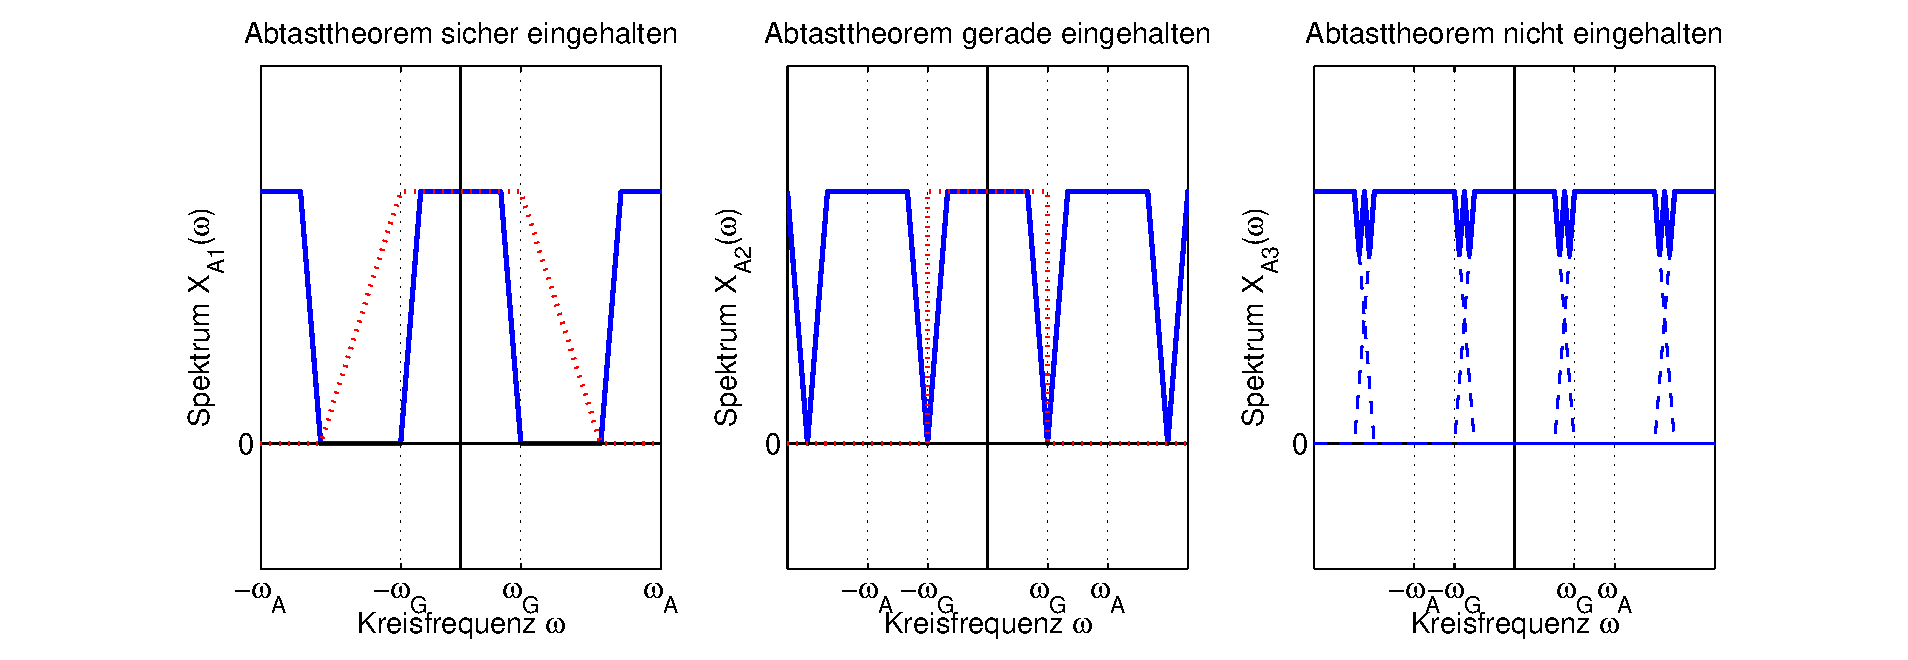
\includegraphics[width=1\textwidth]{Kapitel1/Bilder/image10}}
  \caption{Spektren abgetasteter Signale für genügend gro{\ss}e Abtastfrequenz X$_{A1}$($\omega$), gerade ausreichende Abtastfrequenz X$_{A2}$($\omega$) und für zu kleine Abtastfrequenz X$_{A3}$($\omega$)}
  \label{fig:SpektrenAbgetasteterSignale}
\end{figure}

\noindent
\colorbox{lightgray}{%
\arrayrulecolor{white}%
\renewcommand\arraystretch{0.6}%
\begin{tabular}{ wl{16.5cm} }
{\fontfamily{phv}\selectfont{Beispiel: Abtastrate einer Sound-Karte} }
\end{tabular}%
}\medskip

\noindent Sound-Karten von Computern besitzen einen Analog-Digital-Wandler (ADC). Er wandelt das analoge Signal in ein digitales Signal um. Bei Sound-Karten ist zum einen die Auflösung des ADC wichtig, da sie die Quantisierungsfehler und damit das Rauschen bestimmt. Zweiter wesentlicher Faktor ist die Abtastrate.

\begin{figure}[H]
  \centerline{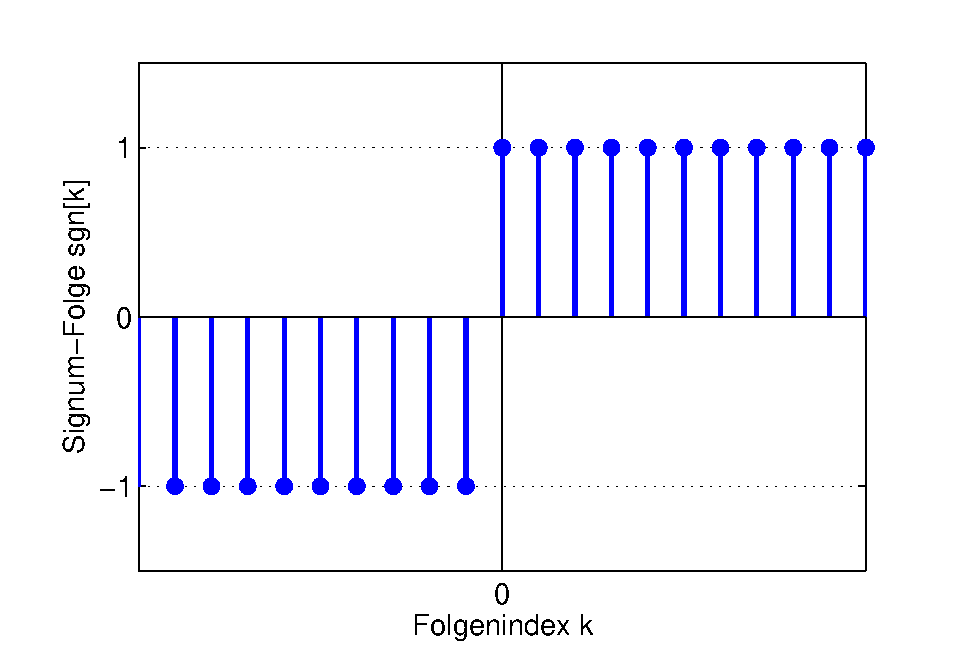
\includegraphics[width=0.5\textwidth]{Kapitel1/Bilder/image11}}
  \caption{Sound-Karte für Personal Computer}
  \label{fig:SoundKarte}
\end{figure}

\noindent Eine Abtastfrequenz f$_{A}$ = 44 kHz ermöglicht die Aufnahme und Wiedergabe bis zu einer theoretischen Bandbreite von 

\begin{equation}\label{eq:twoeighteen}
f_{G} =\frac{f_{A} }{2} =22{\rm \; }kHz
\end{equation}

\noindent Mit der Sound-Karte können damit Musiksignale mit einer maximalen Frequenz von 22 kHz verarbeitet werden.


\subsubsection{Bandbegrenzung des abzutastenden Signals}

\noindent Das Abtasttheorem geht davon aus, dass das Signal bandbegrenzt ist. Reale Signale haben in praktischen Anwendungen aber im Allgemeinen keine harte Bandbegrenzung. Vielmehr ergibt sich ihre Bandbreite aus dem Tiefpassverhalten des Systems, das das Signal generiert, und dem Spektrum von überlagerten Störungen. Um den Einfluss der mangelhaften Bandbegrenzung zu reduzieren, kann ein analoger Tiefpass wie zum Beispiel ein RC-Glied zur Filterung eingesetzt werden. Er verhindert, dass sich in dem Spektrum höhere Frequenzanteile befinden als erwartet, und reduziert damit den Einfluss von Störungen. Das Tiefpass-Filter wird aufgrund seiner Funktion als Anti-Aliasing-Filter bezeichnet. Die Wirkung des Anti-Aliasing-Filters wird in Bild \ref{fig:AntiAliasingFilterWirkung} veranschaulicht.

\begin{figure}[H]
  \centerline{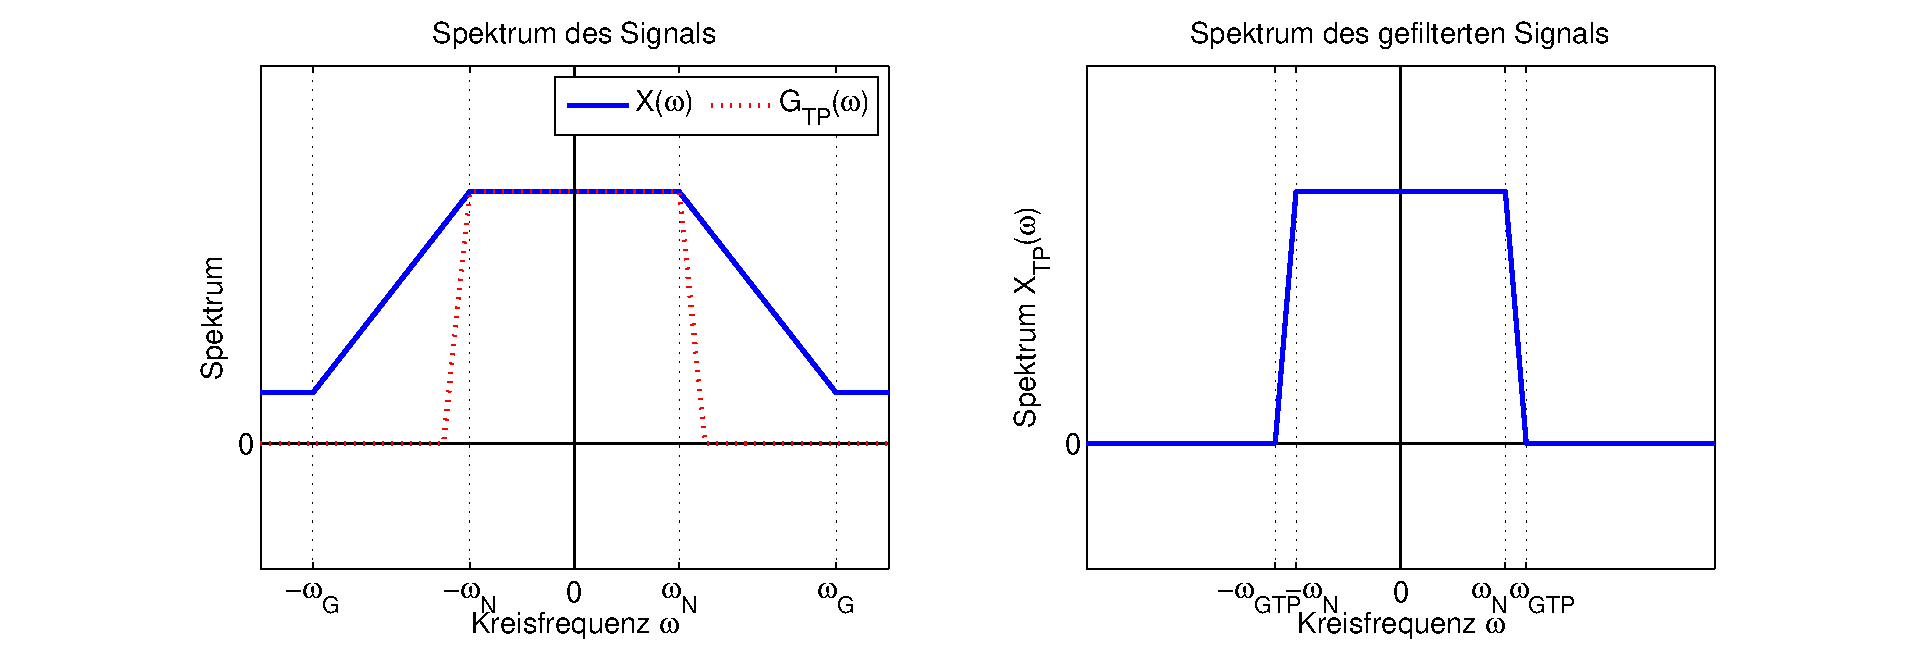
\includegraphics[width=1\textwidth]{Kapitel1/Bilder/image12}}
  \caption{Wirkung des Anti-Aliasing-Filters auf die Bandbegrenzung des Spektrums X($\omega$) des Signals x(t)}
  \label{fig:AntiAliasingFilterWirkung}
\end{figure}

\noindent Das Signal x(t) hat ein Spektrum, dessen Information im Nutzbereich - $\omega_{N} \; \mathrm{<} \; \omega \;  \mathrm{<} \; \omega_{N}$ liegt. Es besitzt aber zum Beispiel aufgrund von Störungen ein breiteres Spektrum. Damit existieren auch oberhalb der als maximal angenommenen Bandbreite $\omega _{G}$ Spektralanteile. Durch den Einsatz eines Tiefpass-Filters, das den Frequenzbereich $\omega \; \mathrm{<}$ - $\omega_{N}$ und den Bereich $\omega \; \mathrm{>} \; \omega_{N}$ dämpft, ergibt sich bei dem neu entstandenen Signal ein Spektrum X$_{TP}$ ($\omega$), das im Nutzbereich dem des ursprünglichen Signals entspricht, im übrigen Bereich aber stärker gedämpft ist. Dieses Signal kann wegen der geringeren Bandbreite $\omega_{GTP} \;  \mathrm{<} \;  \omega_{G}$ mit einer geringeren Frequenz abgetastet werden und der Rauschanteil wird durch die Bandbegrenzung reduziert.

\noindent In technischen Anwendungen wird deshalb praktisch immer ein Eingangstiefpass eingesetzt, das das Spektrum des Eingangssignals auf die notwendige Bandbreite begrenzt. Die Spezifikation von Filtern und ihr Entwurf werden im Teil A dieser Buchreihe diskutiert.\bigskip

\noindent
\colorbox{lightgray}{%
\arrayrulecolor{white}%
\renewcommand\arraystretch{0.6}%
\begin{tabular}{ wl{16.5cm} }
{\fontfamily{phv}\selectfont{Beispiel: Abtastung Drucksensor im Steuergerät} }
\end{tabular}%
}\medskip

\noindent Für die Regelung des Ladedrucks von Turboladern werden Drucksensoren eingesetzt. 

\begin{figure}[H]
  \centerline{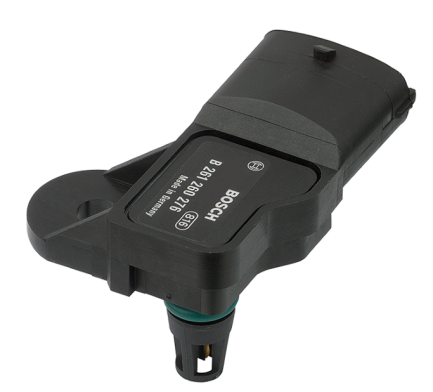
\includegraphics[width=0.3\textwidth]{Kapitel1/Bilder/image13}}
  \caption{Drucksensor zur Messung des Ladedrucks (Bosch)}
  \label{fig:Drucksensor}
\end{figure}

\noindent Der Drucksensor, der den Ladedruck misst, hat besitzt laut Datenblatt eine Zeitkonstante T = 0.1 ms. Das entspricht einer 3dB-Grenzfrequenz von 

\begin{equation}\label{eq:twonineteen}
\omega _{G} =\frac{1}{T} =10{\rm \; }krad/s
\end{equation}

\noindent Das Motor-Steuergerät tastet das Signal mit einer Abtastzeit T${}_{A}$ von 1 ms ab. Es ergibt sich eine Abtastfrequenz von 

\begin{equation}\label{eq:twotwenty}
\omega _{A} =\frac{2\cdot \pi }{T_{A} } =6.283{\rm \; k}rad/s
\end{equation}

\noindent Das Abtasttheorem ist demnach nicht erfällt. Au{\ss}erdem sind dem Sensorsignal Störungen überlagert, die Spektralanteile weit oberhalb der Grenzfrequenz besitzen können. Zur Vermeidung von Aliasing-Effekten wird ein Anti-Aliasing-Filter eingesetzt. Es weist eine Zeitkonstante von T$_{TP}$ = 0.6 ms auf, was einer 3dB-Grenzfrequenz von 

\begin{equation}\label{eq:twotwentyone}
\omega _{TP} =\frac{1}{0.6{\rm \; }ms} ={\rm 1.67\; }krad/s<3.14{\rm \; }krad/s=\frac{\omega _{A} }{2}
\end{equation}

\noindent entspricht. Durch den Einsatz des Tiefpass-Filters wird bei derselben Abtastrate das Abtasttheorem eingehalten. Das Filter hat eine Dämpfung von - 20 dB pro Dekade. Die sich aus der endlichen Steilheit ergebenden Effekte werden in einer Übungsaufgabe diskutiert.

\clearpage


\subsection{Reale Abtastung und Rekonstruktion}

\noindent Die zuvor vorgestellte ideale Abtastfunktion a(t) ist nicht realisierbar, da ideale Impulse technisch nicht erzeugt werden können. Dies liegt an der unendlich kurzen Dauer sowie der unendlichen Steilheit und Höhe von Impulsen. Aus dieser Überlegung ergeben sich die reale Abtastung und die reale Rekonstruktion von Signalen.


\subsubsection{Reale Abtastung eines Signals}

\noindent Reale beziehungsweise technisch realisierbare Abtastsysteme brauchen eine Wandlungszeit T$_{W}$, um aus dem analogen Signal ein zeitdiskretes Signal zu generieren. Die Wandlungszeit ergibt sich zum Beispiel aus einem Ladungstransport oder einem Approximationsprozess, bei dem das Signal als Mittelwert über einen Zeitraum T$_{W}$ durch Integration bestimmt wird. Das real abgetastete Signal x$_{AW}$(t) wird deshalb mit dem Ausdruck

\begin{equation}\label{eq:twotwentytwo}
x_{AW} \left(t\right)=\frac{1}{T_{W} } \cdot \int _{t-T_{W} }^{t}x\left(\tau \right)\, \, d\tau  \cdot \sum _{k=-\infty }^{\infty }\delta \left(t-k\cdot T_{A} \right) =x_{M} \left(t\right)\cdot \sum _{k=-\infty }^{\infty }\delta \left(t-k\cdot T_{A} \right)
\end{equation}

\noindent beschrieben. Es handelt sich um das Produkt von dem gleitenden Mittelwert x${}_{M}$(t) und der idealen Abtastfunktion a(t) im Zeitbereich. Zur Berechnung des Spektrums X${}_{AW}$($\omega$) müssen die Spektren der beiden Signale berechnet werden. Dazu wird das Integral in zwei Summanden zerlegt. 
\begin{equation}\label{eq:twotwentythree}
x_{M} \left(t\right)=\frac{1}{T_{W} } \cdot \int _{t-T_{W} }^{t}x\left(\tau \right)\, \, d\tau  =\frac{1}{T_{W} } \cdot \left(\int _{-\infty }^{t}x\left(\tau \right)\, \, d\tau  -\int _{-\infty }^{t-T_{W} }x\left(t\right)\, \, dt \right)
\end{equation}

\noindent Mit der Integrations- und Verschiebungsregel ergibt sich das zugehörige Spektrum.

\begin{equation}\label{eq:twotwentyfour}
\begin{split}
X_{M} \left(\omega \right) & = \frac{1}{T_{W} } \cdot \left(\frac{1}{j\cdot \omega } \cdot X\left(\omega \right)+\pi \cdot X\left(0\right)\cdot \delta \left(\omega \right)\right)\cdot \left(1-e^{-j\cdot \omega \cdot T_{W} } \right) \\ 
& = \frac{1}{T_{W} } \cdot \left(\frac{1}{j\cdot \omega } \cdot X\left(\omega \right)+\pi \cdot X\left(0\right)\cdot \delta \left(\omega \right)\right)\cdot 2\cdot j\cdot \sin \left(\frac{\omega \cdot T_{W} }{2} \right)\cdot e^{-\frac{j\cdot \omega \cdot T_{W} }{2} }  \\
& \frac{2}{\omega \cdot T_{w} } \cdot\sin \left(\frac{\omega \cdot T_{w}}{2}\right) \cdot X(\omega)\cdot e^{-\frac{j\cdot \omega \cdot T_{W} }{2} } + \frac{\pi\cdot X(0)}{T_{W}}\cdot \delta(\omega) \cdot 2 \cdot j \cdot \sin \left(\frac{\omega \cdot T_{w}}{2}\right)\cdot e^{-\frac{j\cdot \omega \cdot T_{W} }{2} }
\end{split}
\end{equation}

\noindent Da der letzte Summand in Gleichung \eqref{eq:twotwentyfour} null ist, gilt:

\begin{equation}\label{eq:twotwentyfive}
X_{M} \left(\omega \right)=\frac{2}{\omega \cdot T_{W} } \cdot \sin \left(\frac{\omega \cdot T_{W} }{2} \right)\cdot X\left(\omega \right)\cdot e^{-\frac{j\cdot \omega \cdot T_{W} }{2} }
\end{equation}

\noindent Mit dem Spektrum der idealen Abtastfunktion a(t) aus Gleichung \eqref{eq:twonine} und der Multiplikationsregel kann das Spektrum des real abgetasteten Signals berechnet werden zu

\begin{equation}\label{eq:twotwentysix}
\begin{split}
X{}_{AW} \left(\omega \right) & = {\frac{1}{2\cdot \pi } \cdot \left(\frac{2}{\omega \cdot T_{W} } \cdot \sin \left(\frac{\omega \cdot T_{W} }{2} \right)\cdot X\left(\omega \right)\cdot e^{-\frac{j\cdot \omega \cdot T_{W} }{2} } \right)*\left(\frac{2\cdot \pi }{T_{A} } \cdot \sum _{k=-\infty }^{\infty }\delta \left(\omega -k\cdot \omega _{A} \right) \right)} \\ 
& = \frac{1}{T_{A} } \cdot \sum _{k=-\infty }^{\infty }\frac{2}{\left(\omega -k\cdot \omega _{A} \right)\cdot T_{W} } \cdot \sin \left(\frac{\left(\omega -k\cdot \omega _{A} \right)\cdot T_{W} }{2} \right)\cdot X\left(\omega -k\cdot \omega _{A} \right)\cdot e^{-\frac{j\cdot \left(\omega -k\cdot \omega _{A} \right)\cdot T_{W} }{2}} 
\end{split}
\end{equation}

\noindent Wie bei der idealen Abtastung wird das Spektrum mit 1/T${}_{A}$ skaliert und periodisch in $\omega_{A}$ wiederholt. Allerdings wird das Spektrum des zeitkontinuierlichen Signals vor der periodischen Wiederholung mit einem Frequenzgang multipliziert, der sich aus der gleitenden Mittelung ergibt. Allerdings wird das Spektrum des zeitkontinuierlichen Signals vor der periodischen Wiederholung mit dem Spektrum der Fensterfunktion multipliziert. Dieser Vorgang wird in Bild \ref{fig:AbtastprozessRealSpektrum} f\"{u}r eine Wandlungszeiten von  T${}_{W}$ = T${}_{A}$ und T${}_{W}$ = 0.1$\cdot$T${}_{A}$ dargestellt. Die Auswirkung auf das Spektrum im Basisband steigt mit steigender Wandlungszeit. In Analog-Digital-Wandlern wird der Effekt durch geringe Wandlungszeiten klein gehalten und durch den Einsatz inverser Filter kompensiert.

\begin{figure}[H]
  \centerline{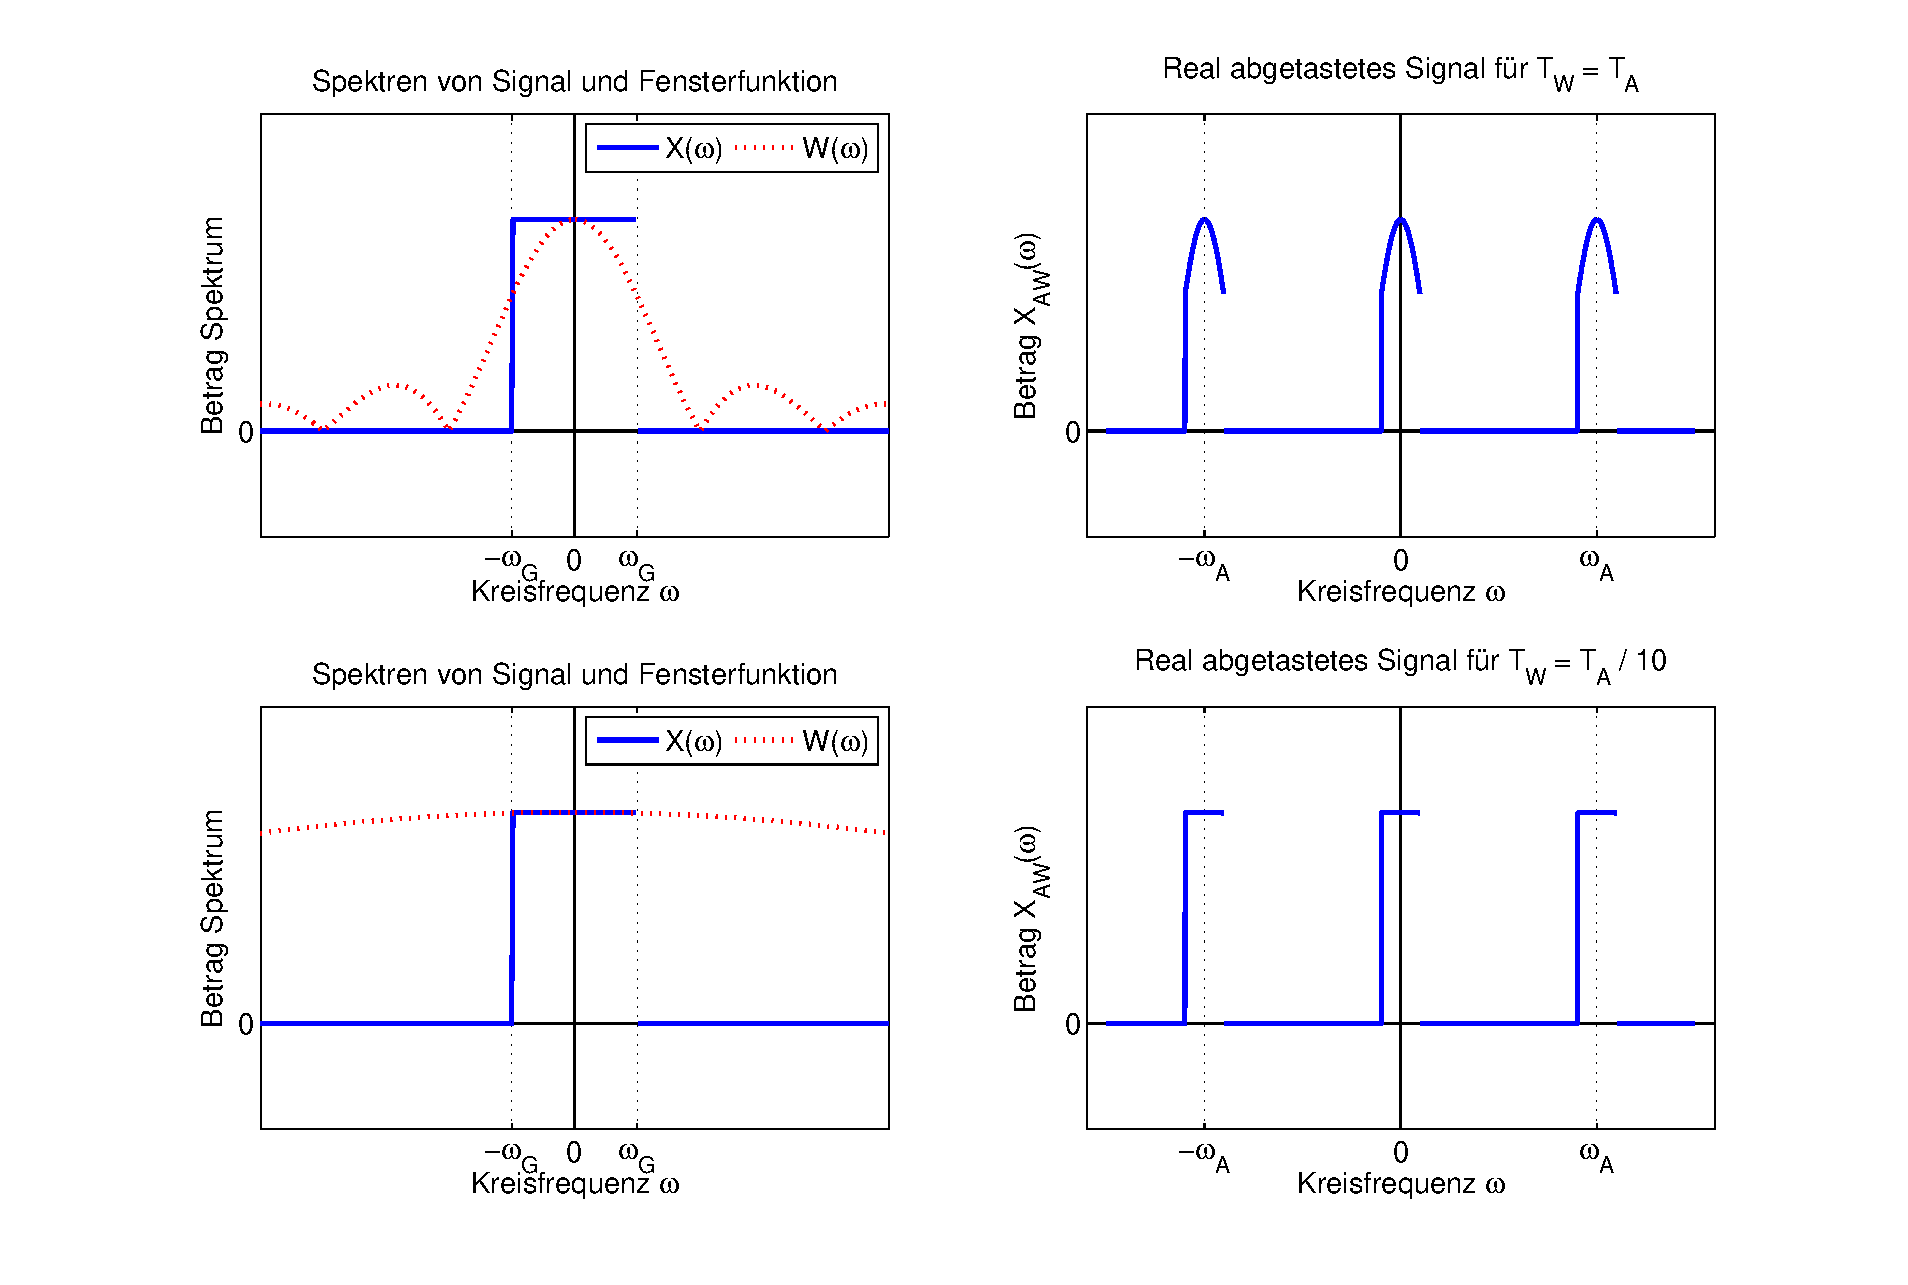
\includegraphics[width=1\textwidth]{Kapitel1/Bilder/image14}}
  \caption{ Darstellung des Spektrums eines realen Abtastprozesses für unterschiedliche Wandlungszeiten T$_{W}$ = T$_{A}$ und T$_{W}$ = 0.1$\cdot$T$_{A}$
}
  \label{fig:AbtastprozessRealSpektrum}
\end{figure}


\subsubsection{Reale Rekonstruktion eines Signals}

\noindent Nach der Abtastung liegen einzelne Abtastwerte vor, die das Signal zu den entsprechenden Abtastzeiten charakterisieren. F\"{u}r einige Anwendungen ist es notwendig, diese zeitdiskreten Signale wieder in zeitkontinuierliche Signale zu wandeln. Die bereits diskutierte ideale Rekonstruktion eines Signals ist wegen des ideal angenommenen Tiefpass-Filters nicht kausal und kann deshalb technisch nicht realisiert werden. Eine technisch realisierbare Rekonstruktion des urspr\"{u}nglichen Signals aus den Abtastwerten wird in zwei Schritten realisiert: 

\begin{itemize}
\item  Erzeugung eines stufenf\"{o}rmigen Ausgangssignals mit einem Halteglied
\item  Tiefpass-Filterung
\end{itemize}

\noindent Die beiden Schritte werden im Zeit- und Frequenzbereich beschrieben. Zur \"{U}bersicht stellt Bild \ref{fig:SignalflussRekonstruktion} den Signalfluss einer realen Signalrekonstruktion bei idealer Signalabtastung dar.

\clearpage
\begin{figure}[H]
  \centerline{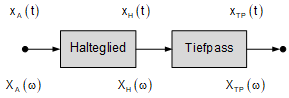
\includegraphics[width=0.4\textwidth]{Kapitel1/Bilder/image15}}
  \caption{Signalfluss zur realen Rekonstruktion}
  \label{fig:SignalflussRekonstruktion}
\end{figure}


{\fontfamily{phv}\selectfont
\noindent\textbf{Erzeugung eines stufenförmigen Ausgangssignals mit einem Halteglied}} \smallskip

\noindent Die einzelnen Abtastwerte stellen das Signal zu den entsprechenden Abtastzeiten dar. Das Halteglied H h\"{a}lt den aktuell g\"{u}ltigen Wert des digitalen Systems am Ausgang fest, bis der n\"{a}chste Abtastwert zur Verf\"{u}gung steht. Dadurch steht zu jedem Zeitpunkt t ein Ausgangssignal zur Verf\"{u}gung und das Signal ist wieder zeitkontinuierlich. Bild \ref{fig:RekonstruktionRealSignal} zeigt an einem Beispiel das abgetastete Signal x${}_{A}$(t) und das Signal x${}_{H}$(t) nach dem Halteglied.

\begin{figure}[H]
  \centerline{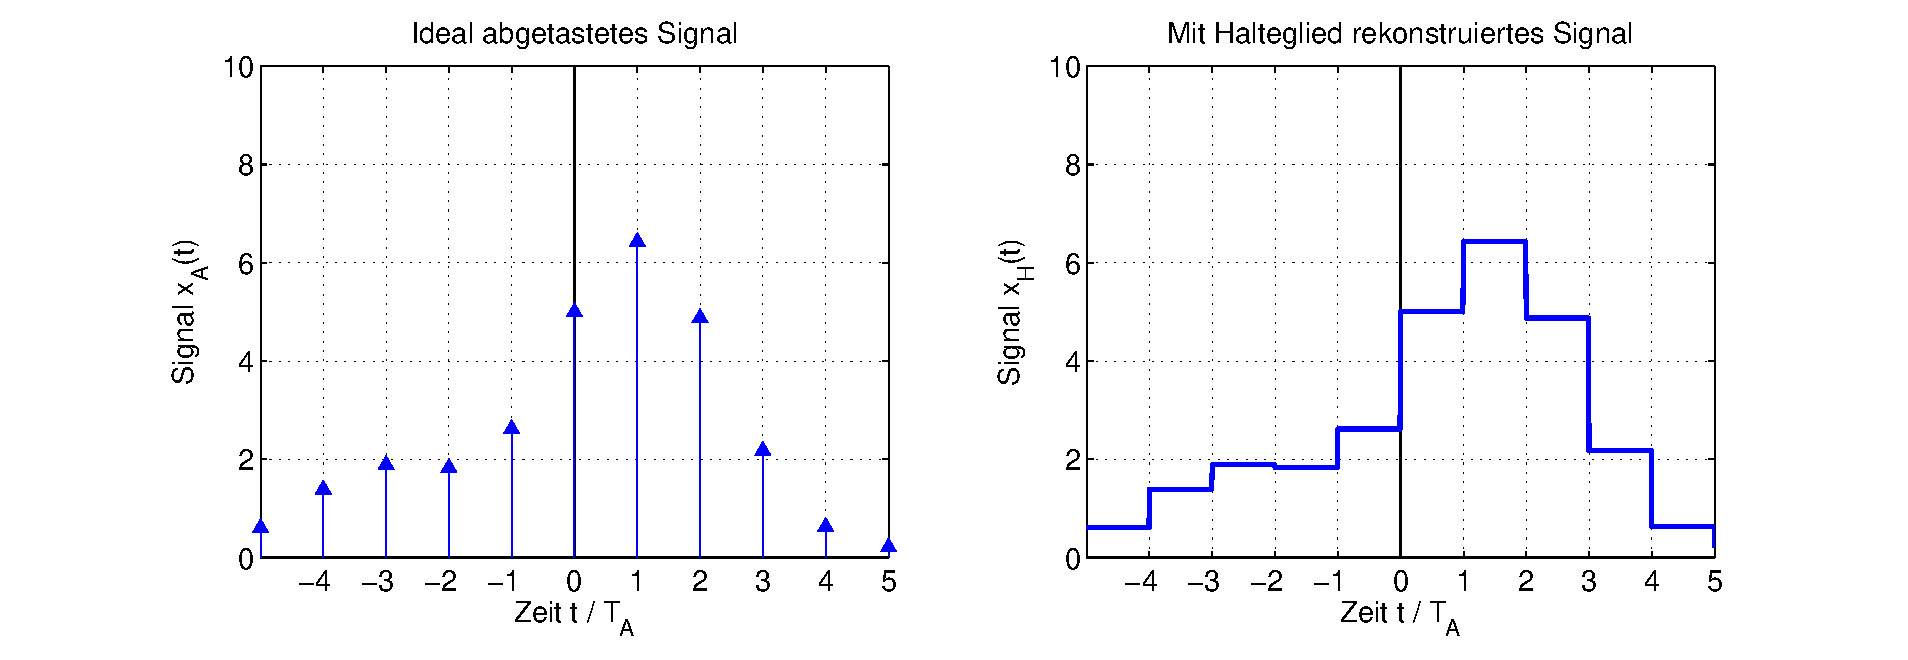
\includegraphics[width=1\textwidth]{Kapitel1/Bilder/image16}}
  \caption{Rekonstruktion eines abgetasteten Signals mit Halteglied}
  \label{fig:RekonstruktionRealSignal}
\end{figure}

\noindent Im Zeitbereich kann das kontinuierliche Signal nach dem Halteglied analog zur realen Wandlung mit Rechteckfunktionen beschrieben werden.

\begin{equation}\label{eq:twotwentyseven}
w\left(t\right)=\frac{1}{T_{W} } \cdot \left(\sigma \left(t\right)-\sigma \left(t-T_{W} \right)\right)
\end{equation}

\noindent Das Signal nach dem Halteglied kann wieder als Faltung ausgedr\"{u}ckt werden.

\begin{equation}\label{eq:twotwentyeight}
\begin{split}
x_{H} \left(t\right) & = \sum _{k=-\infty }^{\infty }x_{A} \left(k\cdot T_{A} \right)\cdot  \left(\sigma \left(t-k\cdot T_{A} \right)-\sigma \left(t-\left(k+1\right)\cdot T_{A} \right)\right) \\ 
& = \left(\sum _{k=-\infty }^{\infty }x\left(k\cdot T_{A} \right)\cdot \delta \left(t-k\cdot T_{A} \right) \right)*\left(\sigma \left(t\right)-\sigma \left(t-T_{A} \right)\right)    
\end{split}
\end{equation}

\noindent Der Faltung der Signale im Zeitbereich entspricht die Multiplikation der Spektren im Frequenzbereich. Das Spektrum des Signals nach dem Halteglied ergibt sich damit aus dem Produkt des Spektrums X${}_{A}$($\omega$) und dem Frequenzgang des Halteglieds H($\omega$).

\begin{equation}\label{eq:twotwentynine}
H\left(\omega \right)=\frac{2}{\omega } \cdot \sin \left(\frac{\omega \cdot T_{A} }{2} \right)\cdot e^{-j\cdot \frac{\omega \cdot T_{A} }{2} }
\end{equation}


\noindent Bild \ref{fig:RekonstruktionRealSpektrum} zeigt das Spektrum des abgetasteten Signals x${}_{A}$(t) und dem Signal x${}_{H}$(t) nach dem Halteglied.

\begin{figure}[H]
  \centerline{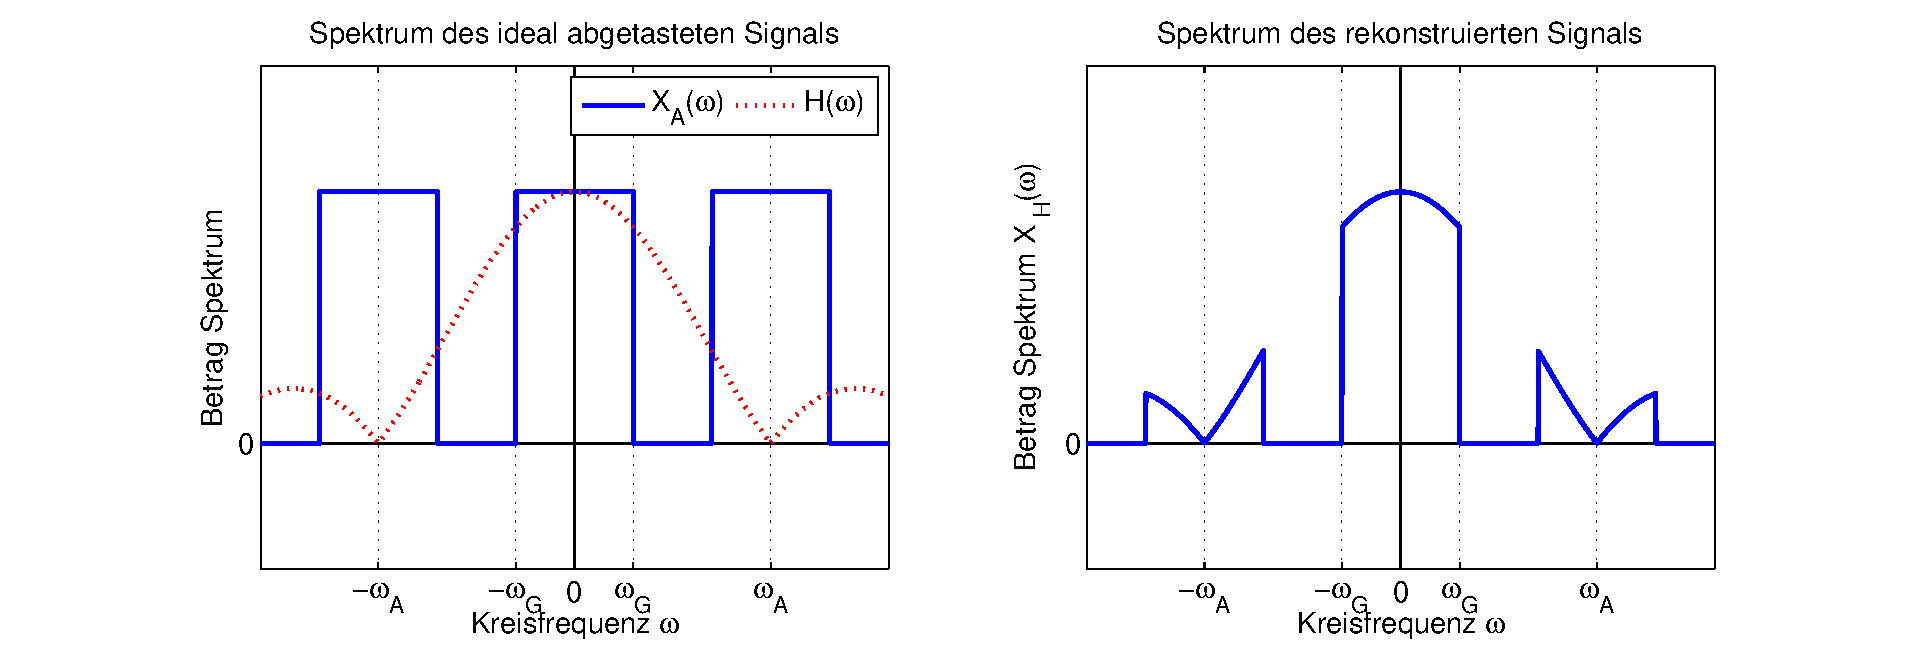
\includegraphics[width=1\textwidth]{Kapitel1/Bilder/image17}}
  \caption{Betrag des Spektrums vom abgetasteten Signal x${}_{A}$(t) und vom Signal x${}_{H}$(t) nach dem Halteglied}
  \label{fig:RekonstruktionRealSpektrum}
\end{figure}

\noindent Durch das Halteglied wird das Spektrum im Bereich der Grenzfrequenz $\omega_{G}$ ged\"{a}mpft. Diese D\"{a}mpfung wirkt sich aber vor allem auf die periodische Fortsetzung des Spektrums aus. \bigskip

{\fontfamily{phv}\selectfont
\noindent\textbf{Filterung des stufenf\"{o}rmigen Signals}} \smallskip

\noindent Zur Vermeidung von Signalspr\"{u}ngen im rekonstruierten Signal wird das Spektrum nach dem Halteglied mit einem geeigneten Filter gefiltert. Mit der \"{U}bertragungsfunktion dem Frequenzgang des Filters G${}_{R}$($\omega$) ergibt sich der Frequenzgang des rekonstruierten Signals x${}_{R}$(t) zu

\begin{equation}\label{eq:twothirty}
X_{R} \left(\omega \right)=X_{A} \left(\omega \right)\cdot \frac{2}{\omega } \cdot \sin \left(\frac{\omega \cdot T_{A} }{2} \right)\cdot e^{-j\cdot \frac{\omega \cdot T_{A} }{2} } \cdot G_{R} \left(\omega \right)
\end{equation}

\noindent Idealerweise w\"{u}rde das Filter die Abweichungen im Basisband des Nutzsignals - $\omega_{N} \mathrm{<} \omega \mathrm{<} \omega_{N}$ kompensieren und die Frequenzanteile ober- und unterhalb des Basisbandes vollst\"{a}ndig eliminieren. Bild \ref{fig:RekonstruktionTiefpassSpektrum} verdeutlicht diesen Ansatz.

\begin{figure}[H]
  \centerline{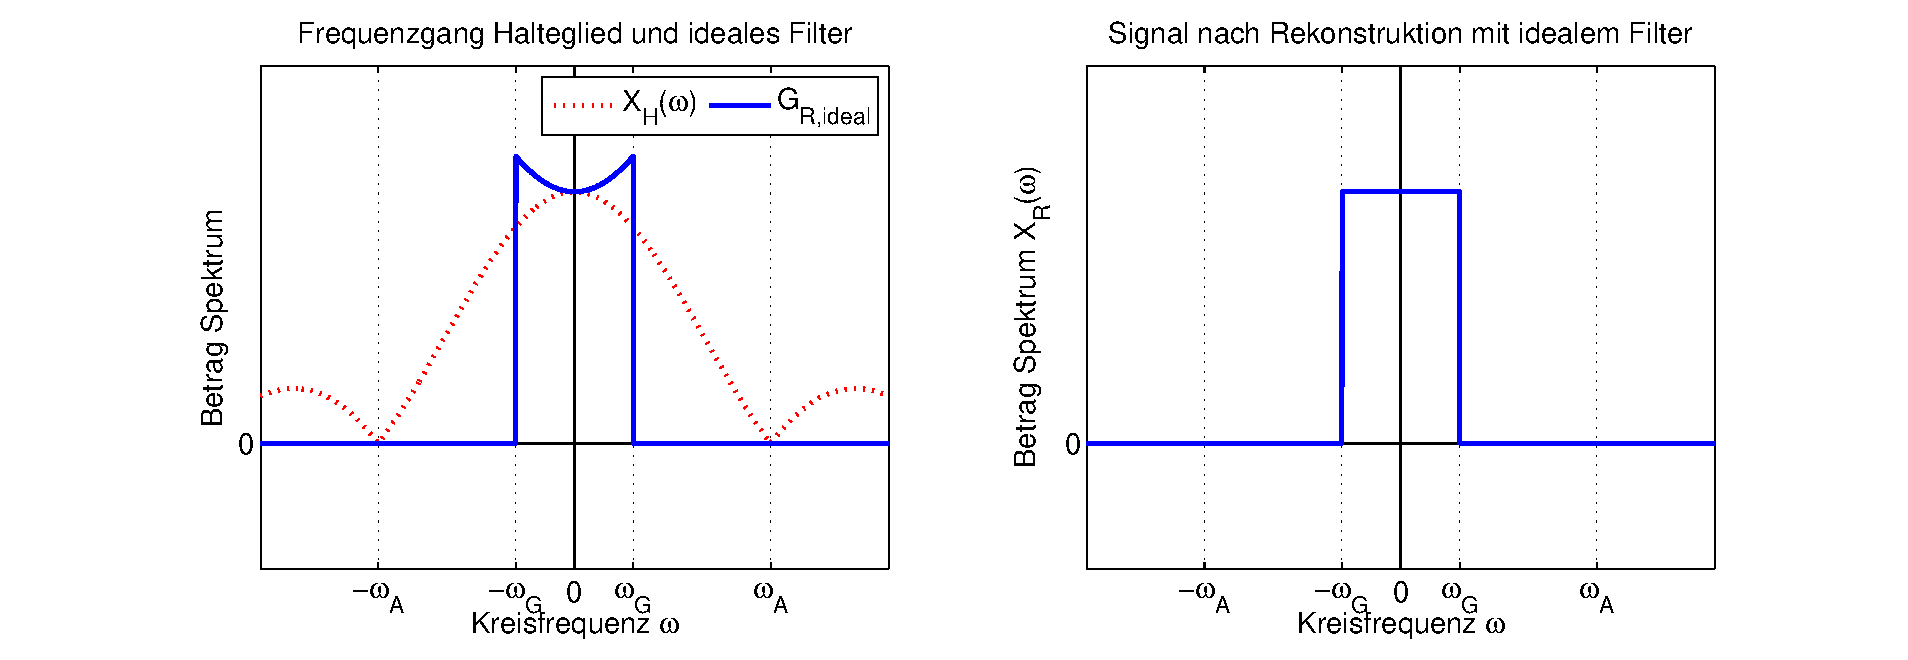
\includegraphics[width=1\textwidth]{Kapitel1/Bilder/image18}}
  \caption{Ideales Filter zur Rekonstruktion eines abgetasteten Signals}
  \label{fig:RekonstruktionTiefpassSpektrum}
\end{figure}

\clearpage

\noindent Dieses ideale Filter ist wegen der idealen Flankensteilheit nicht realisierbar. Reale Filter beschr\"{a}nken sich auf eine endliche Flankensteilheit. Eine M\"{o}glichkeit, die erforderliche Flankensteilheit zu senken, ist eine Steigerung der Abtastrate f${}_{A}$. Dieser Vorgang wird als \"{U}berabtastung oder Oversampling bezeichnet. Durch die h\"{o}here Abtastrate werden zwei Effekte erzielt:

\begin{itemize}
\item  Die Trennung der periodischen Spektren ist gr\"{o}{\ss}er. Dadurch kann die Ordnung des Filters zur Signal-Rekonstruktion reduziert werden.

\item  Mit h\"{o}herer Abtastrate liegt der Nutzbereich des Signals immer mehr im flachen Bereich der \"{U}bertragungsfunktion des Halteglieds, sodass eine Kompensation des Frequenzgangs des Halteglieds nicht weiter notwendig ist.
\end{itemize}

\noindent Die zum Halteglied inverse Charakteristik im Durchlassbereich kann \"{u}ber ein digitales Filter erreicht werden, der als Teil der digitalen Signalverarbeitung realisiert wird. 


\subsubsection{Totzeit bei der realen Signalabtastung}

\noindent In den vorangegangenen Abschnitten wird der Abtastvorgang hinsichtlich der Auswirkung auf den Betrag des Spektrums diskutiert. Die \"{U}bertragungsfunktionen weisen aber immer auch eine Phasenverschiebung auf. Die gesamte Phasenverschiebung ergibt sich bei der realen Abtastung nach den obigen Darstellungen aus den Totzeiten des Wandlers und des Halteglieds.


\begin{equation}\label{eq:twothirtyone}
T_{T} =\frac{T_{W} }{2} +\frac{T_{A} }{2}
\end{equation}

\noindent Dazu kommen die Phase des Anti-Aliasing-Filters und des Tiefpass-Filters zur Signalrekonstruktion, sodass gegen\"{u}ber dem Eingangssignal eine teilweise erhebliche Signalverz\"{o}gerung entsteht. Die Zeitverz\"{o}gerung sowie das Einschwingverhalten des rekonstruierten Signals werden an einem Beispiel verdeutlicht.\bigskip

\noindent
\colorbox{lightgray}{%
\arrayrulecolor{white}%
\renewcommand\arraystretch{0.6}%
\begin{tabular}{ wl{16.5cm} }
{\fontfamily{phv}\selectfont{Beispiel: Signalrekonstruktion} }
\end{tabular}%
}\medskip

\noindent Ein Signal der Form 

\begin{equation}\label{eq:twothirtytwo}
x\left(t\right)=5\cdot e^{-0.1\cdot t^{2} } \cdot \left(1+0.5\cdot \sin \left(t\right)\right)\cdot \left(\sigma \left(t+5\right)-\sigma \left(t-5\right)\right)
\end{equation}

\noindent wird mit einer Abtastzeit von T$_{A}$ = 1 abgetastet, das System besitzt eine Wandlungszeit von T$_{W}$ = 1. Es entstehen die in Tabelle \ref{tab:twoone} dargestellten Abtastwerte.

\clearpage
\begin{table}[H]
\setlength{\arrayrulewidth}{.1em}
\caption{Tabellarische Übersicht über Signaleigenschaften für Signalfolgen}

\setlength{\fboxsep}{0pt}%
\colorbox{lightgray}{%
\arrayrulecolor{white}%
\begin{tabular}{| c | c | c | c | c | c | c | c | c | c | c | c |}
\hline
\parbox[c][0.45in][c]{0.45in}{\smallskip\centering\textbf{\fontfamily{phv}\selectfont{T/T${}_{A}$}}} & 
\parbox[c][0.37in][c]{0.37in}{\centering{-5}} & 
\parbox[c][0.37in][c]{0.37in}{\centering{-4}} & 
\parbox[c][0.37in][c]{0.37in}{\centering{-3}} & 
\parbox[c][0.37in][c]{0.37in}{\centering{-2}} & 
\parbox[c][0.37in][c]{0.37in}{\centering{-1}} & 
\parbox[c][0.37in][c]{0.37in}{\centering{0}} & 
\parbox[c][0.37in][c]{0.37in}{\centering{1}} & 
\parbox[c][0.37in][c]{0.37in}{\centering{2}} & 
\parbox[c][0.37in][c]{0.37in}{\centering{3}} & 
\parbox[c][0.37in][c]{0.37in}{\centering{4}} & 
\parbox[c][0.37in][c]{0.37in}{\centering{5}}\\  \hline
\parbox[c][0.45in][c]{0.45in}{\smallskip\centering\textbf{\fontfamily{phv}\selectfont{x(k$\cdot$T${}_{A}$)}}} & 
\parbox[c][0.37in][c]{0.37in}{\centering{0.607}} & 
\parbox[c][0.37in][c]{0.37in}{\centering{1.392}} & 
\parbox[c][0.37in][c]{0.37in}{\centering{1.889}} & 
\parbox[c][0.37in][c]{0.37in}{\centering{1.828}} & 
\parbox[c][0.37in][c]{0.37in}{\centering{2.621}} & 
\parbox[c][0.37in][c]{0.37in}{\centering{5.000}} & 
\parbox[c][0.37in][c]{0.37in}{\centering{6.428}} & 
\parbox[c][0.37in][c]{0.37in}{\centering{4.875}} & 
\parbox[c][0.37in][c]{0.37in}{\centering{2.176}} & 
\parbox[c][0.37in][c]{0.37in}{\centering{0.628}} & 
\parbox[c][0.37in][c]{0.37in}{\centering{0.214}}\\ \hline

\end{tabular}%
}
\label{tab:twoone}
\end{table}


\noindent Die Abtastwerte werden über ein Halteglied und einen Tiefpass mit einer Zeitkonstante T${}_{TP}$ = 0.5 rekonstruiert. Bild \ref{fig:RekonstruktionRealSignalTiefpass} zeigt das analoge Signal x(t) und das durch Abtastung und Rekonstruktion erzeugte Signal x${}_{TP}$(t) bei Verwendung eines Tiefpass erster Ordnung.

\begin{figure}[H]
  \centerline{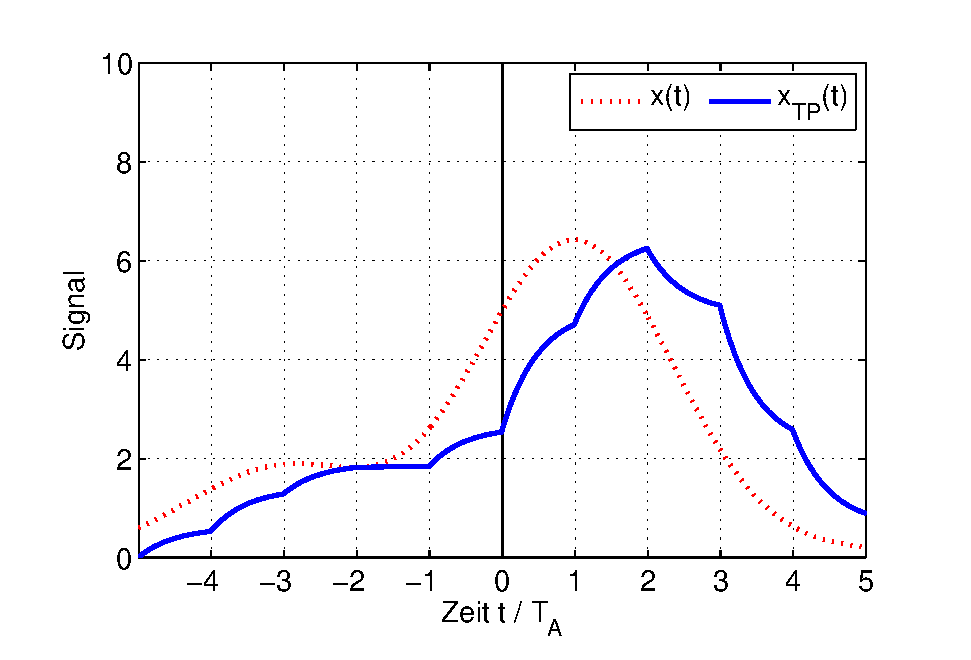
\includegraphics[width=0.5\textwidth]{Kapitel1/Bilder/image19}}
  \caption{Vergleich eines Zeitsignals x(t) und der realen Rekonstruktion des abgetasteten Signals mit einem Tiefpass erster Ordnung}
  \label{fig:RekonstruktionRealSignalTiefpass}
\end{figure}

\noindent Das rekonstruierte Signal weist zum einen eine Verzögerung von

\begin{equation}\label{eq:twothirtythree}
T_{T} =\frac{T_{W} }{2} +\frac{T_{A} }{2} =\frac{T_{A} }{2} +\frac{T_{A} }{2} =T_{A}
\end{equation}

\noindent auf. Au{\ss}erdem ist das Einschwingen des Tiefpasses nach jedem Quantisierungsschritt zu erkennen. 

\noindent Diese Signalverzögerung T${}_{T}$ ist insbesondere bei Regelungssystemen kritisch anzusehen. Auch in dieser Beziehung ist eine hohe Abtastrate, die wegen kleiner Abtastzeit und Wandlungszeit zu einer Verringerung der Totzeit führt, vorteilhaft.

\InsertBoxL{0}{
\includegraphics[scale=0.5]{Code.JPG}} 
\textcolor{white}{.}\newline
\noindent Im Online-Portal \textit{Systemtheorie Online} verdeutlicht die \textit{Applikation Signalabtastung und Signal-
rekonstruktion} grafisch, welche Effekte durch Anti-Aliasing-Filter, reale Abtastung und reale Rekon-struktion entstehen.\newline    

\clearpage

\subsection{Literatur}


\subsubsection{Literaturstellen mit besonders anschaulicher Darstellung}

\begin{tabular}{|p{0.8in}|p{5.7in}|} \hline 
[Lyon04] & Lyons, Richard G.: Understanding Digital Signal \newline Processing,Prentice Hall, New Jersey, 2004 \\ \hline 
[Stea99] & Stearns, Samuel: Digitale Verarbeitung analoger Signale,\newline 7. Auflage, Oldenbourg Verlag M\"{u}nchen, 1999 \\ \hline 
\end{tabular}


\subsubsection{Literaturstellen mit praktischen Anwendungen}

\begin{tabular}{|p{0.8in}|p{5.7in}|} \hline 
[Wern08] & Werner, Martin: Signale und Systeme,\newline
Vieweg Studium Technik, Wiesbaden, 2008 \\\hline 
[Meye08] & Meyer, Martin: Signalverarbeitung -- Analoge und digitale Signal, Systeme und Filter,\newline 
Vieweg Studium Technik, Wiesbaden, 2008 \\  \hline 
\end{tabular}


\subsubsection{ Weiterf\"{u}hrende Literatur}

\begin{tabular}{|p{0.8in}|p{3.7in}|} \hline 
[Oppe04] & Oppenheim, Alan: Zeitdiskrete Signalverarbeitung,\newline 2. \"{u}berarbeitete Auflage, Pearson Studium, 2004 \\ \hline 
[Kamm98] & Kammeyer, Karl: Digitale Signalverarbeitung,\newline B.G. Teubner Stuttgart, 1998 \\ \hline 
\end{tabular}
